\chapter{积分算法的设计及基本分析}
对于结构动力学运动方程
\begin{equation}
\bm{M}\ddot{\bm{U}}(t)+\bm{C}\dot{\bm{U}}(t)+\bm{KU}(t)=\bm{F}(t)\label{eq:ch2DyEq}
\end{equation}
的数值求解及其数值算法的设计分析,许多的基本概念借助于数学上对一阶微分方程
\begin{equation}
\dot{y}(t)=f(y,t)\label{eq:ch2Firsty}
\end{equation}
的数值算法的设计分析,如数值算法的相容性、稳定性和收敛性等。事实上,结构动力学运动方程(\ref{eq:ch2DyEq})本质上就是一个二阶的线性微分方程,通过引入速度为独立的变量,可以将其二阶微分形式降维为具有形如(\ref{eq:ch2Firsty})形式的更高阶一阶微分方程。因此,在这一节主要针对(\ref{eq:ch2Firsty})进行数值算法性能指标分析,如果一些定义对于二阶微分方程有差异,再具体指出。

由于广义线性法是求解微分方程(\ref{eq:ch2Firsty})更具一般性的方法,因此本节先通过最简单的数值算法(Euler法)分析引出广义线性法,而后后续的算法性能分析都尽可能在广义线性的基础上进行定义及分析。而常见的线性多步法和Runge-Kutta法将是由其特例导出。

\section{广义线性法}
在20世纪初.Euler在他的著作中,针对如下自治的一阶微分方程
\begin{equation}
\dot{y}(t)=f(y(x))\label{eq:ch2FirstAuto}
\end{equation}
带有合适的初始条件$y(x_0)=y_0\in\mathbb{X}$的数值求解,给出了如下的数值格式
\begin{equation}
y_n=y_{n-1}+h_nf(y_{n-1}),\qquad n=1,2,\cdots\label{eq:ch2Euler}
\end{equation}
对于每一个给定的$n$值,其$y_n$都可以根据上式由$y_{n-1}$计算得到。同时,$h_n$为在第$n$的积分步长,一般情况下没必要要求在整个积分过程中相等,亦即变时间步长积分。但在本文整个分析过程中,我们假定其数值算法都是在相等的时间步长内进行积分及计算的。亦即
\begin{equation}
h_n\equiv h\qquad n=1,2,\cdots
\end{equation}

显然,该数值格式的优劣很大程度依赖于积分步长$h$以及等式(\ref{eq:ch2FirstAuto})右端项$f(y)$随变量$y$的变化快慢程度。而后者通常由$f(y)$满足的Lipschitz常数$L$来度量。同时,我们也需要提及该条件也保证了微分方程(\ref{eq:ch2FirstAuto})解的存在唯一性。于是,我们在本全文中都假定分析的微分方程都满足该Lipschitz条件。关于该条件的对其微分方程解的存在唯一性的证明,读者可以翻阅任意一本常微分方程的书籍都可以查到。这里不再做过多累述。

事实上,Euler格式(\ref{eq:ch2Euler})简单易用,但它却是条件稳定的且只有一阶精度。在很多时候,并不是很实用。因此,后续许多学者提出了很多改进Euler格式的算法。其中,至少有两个策略进行改进Euler方法
\begin{itemize}
\item[\ddag] 单步内使用更多、更复杂的计算,如Runge-Kutta法。
\item[\ddag] 使用更多已知节点的逼近值。如线性多步法。
\item[\ddag] 更高阶导数值的使用。如Rosenbrock方法。
\item[\ddag] 多步-多级-多导数方法。如拟Runge-Kutta方法。
\end{itemize}

从简单的Euler格式出发,我们可以建立如图\ref{Fig:ch2GeneraAxis}的改进策略坐标系
\begin{figure}[htpb]
\centering
\begin{tikzpicture}[xscale=1.2,yscale=1.2]
\draw [thin,->] (0,0) -- (2,1) node [align=center,below right] {每步更多的\\ 计算量};
\draw [thin,->] (0,0)--(-2,1.5) node [align=center,below left] {更多的\\ 已知节点值};
\draw [thin,->] (0,0)--(0,2) node [left] {$y$的导数};
\draw [thin,->] (0,2) -- (0,4) node [left] {$f$的导数};
%============================================
\draw [thin,fill,red] (0,0) circle [radius = 0.03] node [below] {Euler格式};
\end{tikzpicture}
\bicaption[Fig:ch2GeneraAxis]{}{Euler格式的改进策略示意图}{Fig.$\!$}{Generalizations of the Euler method}
\end{figure}

在图\ref{Fig:ch2GeneraAxis}的坐标系下,现阶段的大多数的数值算法都可以被建立在这个三维算法格式空间中,如图\ref{Fig:ch2GeneraEuler}所示。
\begin{figure}[htpb]
\centering
\begin{tikzpicture}[xscale=1.2,yscale=1.2]
\draw [thin] (0,0) -- (2.5,1) node [right] {Runge-Kutta法};
\draw [thin] (0,0)--(-2,1.5) node [left] {线性多步法};
\draw [thin,dashed] (-2,1.5)--(0.5,2.5);
\draw [thin,dashed] (2.5,1) -- (0.5,2.5);
%============================================
\draw [thin] (0,3) node [left] {泰勒级数法} -- (2.5,4);
\draw [thin] (0,3)--(-2,4.5) node [left] {Obreshkov方法};
\draw [thin,dashed] (-2,4.5)--(0.5,5.5);
\draw [thin,dashed] (2.5,4) -- (0.5,5.5);
%--------------------------------
\draw [thin] (0,3) -- (0,0);
\draw [thin] (2.5,4) -- (2.5,1);
\draw [thin] (-2,4.5) -- (-2,1.5);
\draw [thin,dashed] (0.5,2.5) -- (0.5,5.5);
%=-==========================================
\draw [thin] (0,6) -- (2.5,7) node [right] {Rosenbrock方法};
\draw [thin] (0,6)--(-2,7.5);
\draw [thin] (-2,7.5)--(0.5,8.5);
\draw [thin] (2.5,7) -- (0.5,8.5);
%--------------------------------
\draw [thin] (0,6) -- (0,3);
\draw [thin] (2.5,7) -- (2.5,4);
\draw [thin] (-2,7.5) -- (-2,4.5);
\draw [thin,dashed] (0.5,5.5) -- (0.5,8.5);
%=-==========================================
\draw [thin,fill,red] (0,0) circle [radius = 0.03] node [below] {Euler格式};
\draw [thin,fill,blue] (0.5,2.5) circle [radius = 0.03] node [right] {广义线性法};
\draw [thin,fill] (0,3) circle [radius = 0.03];
\draw [thin,fill] (2.5,7) circle [radius = 0.03];
\draw [thin,fill] (-2,4.5) circle [radius = 0.03];
\draw [thin,fill] (2.5,1) circle [radius = 0.03];
\draw [thin,fill] (-2,1.5) circle [radius = 0.03];
\end{tikzpicture}
\bicaption[Fig:ch2GeneraEuler]{}{Euler格式的改进算法框架}{Fig.$\!$}{Generalized formworks of the Euler method}
\end{figure}
于是,可以知道广义线性法是线性多步法和Runge-Kutta法的结合,更是Euler格式的一般化推广。同时,从该图可以知道,广义线性法并不能包括所有的数值格式,它仅仅是现阶段数值算法的一大类。

广义线性方法即结合了线性多步法的多值特点,又使用了Runge-Kutta方法的多级属性。并且它首次由Butcher教授在1966年提出\cite{Butcher1966b}。下面提及的广义线性法的矩阵表示形式则是由Burrage和Butcher在1980年引入而来\cite{Burrage1980b}。

假定在单步内进行转换的量有$r$个。在第$n$步的开始,这$r$个量被表示为$y_1^{[n-1]},y_2^{[n-1]},\cdots,y_r^{[n-1]}$。当第$n$步完成计算时,对应的$r$量分别为$y_1^{[n]},y_2^{[n]},\cdots,y_r^{[n]}$,并且这些量将作为下一个时间步内的起始值进行后续计算。同时,在单步内计算的$s$个级数值$Y_1,Y_2,\cdots,Y_s$所对应的级数导数值为$F_1,F_2,\cdots,F_S$。为了表示方便,引入如下的$r$或$s$维向量表示,即
\begin{equation}
y^{[n-1]}=\begin{bmatrix}
y_1^{[n-1]}\\
y_2^{[n-1]}\\
\vdots\\
y_r^{[n-1]}
\end{bmatrix},\quad
y^{[n]}=\begin{bmatrix}
y_1^{[n]}\\
y_2^{[n]}\\
\vdots\\
y_r^{[n]}
\end{bmatrix},\quad
Y^{[n]}=\begin{bmatrix}
Y_1^{[n]}\\
Y_2^{[n]}\\
\vdots\\
Y_s^{[n]}
\end{bmatrix},\quad
F(Y^{[n]})=\begin{bmatrix}
f(Y_1^{[n]})\\
f(Y_2^{[n]})\\
\vdots\\
f(Y_s^{[n]})
\end{bmatrix}
\end{equation}

类似于Runge-Kutta方法,级数值$Y_i$是依赖于级数导数值$F_i$的线性组合来计算,但是现在的广义线性法将其推广为不仅依赖于级数导数值的线性组合,也依赖于前述已知节点逼近值$y_i$的线性组合。即
\begin{equation}
Y_i=\sum_{j=1}^{s}ha_{ij}f(Y_j^{[n]})+\sum_{j=1}^{r}u_{ij}y_j^{[n-1]},\qquad i=1,2,\cdots,s
\end{equation}
同理,对于输出量$y_i^{[n]}$也是不仅线性依赖于各个级数导数值$F_i=f(Y_i)$而且也是线性依赖于前述已知节点逼近值$y_i$,即
\begin{equation}
y_i^{[n]}=\sum_{j=1}^{s}hb_{ij}f(Y_j^{[n]})+\sum_{j=1}^{r}v_{ij}y_j^{[n-1]},\qquad i=1,2,\cdots,r
\end{equation}

令$A=[a_{ij}]_{s\times s},U=[u_{ij}]_{s\times r},B=[b_{ij}]_{r\times s}$以及$V=[v_{ij}]_{r\times r}$,同时使用Kronecker积符号($\otimes$),广义线性法则可以表示为
\begin{align}
Y^{[n]}&=h(A\otimes I)F(Y^{[n]})+(U\otimes I)y^{[n-1]}\\
y^{[n]}&=h(B\otimes I)F(Y^{[n]})+(V\otimes I)y^{[n-1]}
\end{align}
其中,$I$表示维度相容的单位矩阵。而Kronecker积定义如下,若$A\in\mathbb{R}^{m_1\times n_1}$和$B\in\bm{R}^{m_2\times n_2}$,则有
\begin{equation}
A\otimes B=\begin{bmatrix}
a_{11} B&&a_{12}B&&\cdots && a_{1,n_1} B\\
a_{21}B&&a_{22}B&&\cdots && a_{2,n_1}B\\
\vdots &&\vdots && &&\vdots\\
a_{m_1,1}B &&a_{m_1,2}B&&\cdots &&a_{m_1,n_1}B
\end{bmatrix}\in\mathbb{R}^{m_1m_2\times n_1n_2}
\end{equation}
进一步,广义线性法可以被表达为如下形式
\begin{equation}
\begin{bmatrix}
\begin{array}{c}
Y^{[n]}\\ \hline
y^{[n]}
\end{array}
\end{bmatrix}=\begin{bmatrix}
\begin{array}{c|c}
A\otimes I & U\otimes I \\ \hline
B\otimes I & V\otimes I
\end{array}
\end{bmatrix}\begin{bmatrix}
\begin{array}{c}
hF(Y^{[n]})\\ \hline
y^{[n-1]}
\end{array}
\end{bmatrix}\label{eq:ch2GLM}
\end{equation}

通常情况下,广义线性法的数值性能就被这四个矩阵所决定,即$A,U,B$和$V$。因此对于一个广义线性法,可以用如下的分块矩阵刻画
\begin{equation}
\begin{bmatrix}
\begin{BMAT}[5pt]{c:c}{c:c}
	\bm{A} & \bm{U} \\
	\bm{B} & \bm{V}
\end{BMAT}
\end{bmatrix}
\end{equation}

当四个矩阵取值不同时,对应着不同的广义线性法。特别地,线性多步法和Runge-Kutta都是其特例。
\subsection{线性多步法}
考虑对于一阶微分方程(\ref{eq:ch2Firsty})的$k$步线性多步法
\begin{equation}
y_n=\sum_{j=1}^{k}\alpha_jy_{n-j}+h\sum_{j=0}^{k}\beta_jf(y_{n-j})\label{eq:ch2lms}
\end{equation}
令$Y^{[n]}=y_n$,并且
\begin{subequations}
\begin{align}
y^{[n]}&=[y_n,y_{n-1},\cdots,y_{n-k+1},hf(y_n),hf(y_{n-1}),\cdots,hf(y_{n-k+1})]^{\text{T}}\\
y^{[n-1]}&=[y_{n-1},y_{n-2},\cdots,y_{n-k},hf(y_{n-1}),hf(y_{n-2}),\cdots,hf(y_{n-k})]^{\text{T}}
\end{align}
\end{subequations}
于是,对于$k$步的线性多步法(\ref{eq:ch2lms})可以写成广义线性法的形式\cite{Burrage1980b},即$r=2k,s=1$
\begin{equation}
\begin{bmatrix}
\begin{BMAT}[5pt]{c:c}{c:c}
A & U\\
B & V
\end{BMAT}
\end{bmatrix}=\begin{bmatrix}
\begin{BMAT}[5pt]{c:cccccccc}{c:cccccccc}
\beta_0 & \alpha_1 & \cdots & \alpha_{k-1} & \alpha_k & \beta_1 & \cdots & \beta_{k-1} & \beta_k\\
\beta_0 & \alpha_1 & \cdots & \alpha_{k-1} & \alpha_k & \beta_1 & \cdots & \beta_{k-1} & \beta_k\\
0 & 1 & \cdots & 0 & 0 & 0 & \cdots & 0 & 0\\
\vdots & \vdots & \ddots &\vdots & \vdots &\vdots &\ddots &\vdots &\vdots \\
0 & 0 &\cdots & 1 & 0 &0 &\cdots & 0 & 0 \\
1 & 0 & \cdots & 0 & 0 & 0 & \cdots & 0 & 0\\
0 & 0 & \cdots & 0 & 0 & 1 & \cdots & 0 & 0\\
\vdots & \vdots & \ddots &\vdots & \vdots &\vdots &\ddots &\vdots &\vdots \\
0 & 0 & \cdots & 0 & 0 & 0 & \cdots & 1 & 0
\end{BMAT}
\end{bmatrix}
\end{equation}
特别地,$k$步的线性多步法(\ref{eq:ch2lms})也可以写成$r=k,s=1$的广义线性法形式\cite{Butcher2006f}。文\inlinecite{Butcher2006f}中定义
\begin{equation}
y_i^{[n-1]}=\sum_{j=k-i+1}^{k}(\alpha_jy_{n+k-i-j}+h\beta_jf(y_{n+k-i-j})),\quad i=1,2,\cdots,k\label{eq:ch2skeel}
\end{equation}
其实,公式(\ref{eq:ch2skeel})在文献\inlinecite{Skeel1979a}就已经被提出来了,只不过没有涉及广义线性法的应用。于是,线性多步法(\ref{eq:ch2lms})则可以写成如下形式
\begin{equation}
y_n=h\beta_0f(y_n)+\sum_{j=1}^{k}(\alpha_jy_{n-j}+h\beta_jf(y_{n-j}))=h\beta_0f(y_n)+y_k^{[n-1]}
\end{equation}
进一步,在$n$步结束时有
\begin{equation}
\begin{aligned}
y_i^{[n]}&=\sum_{j=k-i+1}^{k}(\alpha_jy_{n+1+k-i-j}+h\beta_jf(y_{n+1+k-i-j}))\\
&=\alpha_{k-i+1}y_n+h\beta_{k-i+1}f(y_n)+\sum_{j=k-i+2}^{k}(\alpha_jy_{n+1+k-i-j}+h\beta_jf(y_{n+1+k-i-j}))\\
&=(\alpha_{k-i+1}\beta_0+\beta_{k-i+1})hf(y_n)+\alpha_{k-i+1}y_k^{[n-1]}+y_{i-1}^{[n-1]}
\end{aligned}
\end{equation}
其中,$i=1,2,\cdots,k$。线性多步法(\ref{eq:ch2lms})的另外一种广义线性法的表出形式为
\begin{equation}
\begin{bmatrix}
\begin{BMAT}[5pt]{c:c}{c:c}
A & U\\
B & V
\end{BMAT}
\end{bmatrix}=\begin{bmatrix}
\begin{BMAT}[5pt]{c:cccccc}{c:cccccc}
\beta_0 & 0 & 0 & 0 & \cdots & 0 & 1\\
\alpha_k\beta_0+\beta_k & 0 & 0 & 0 & \cdots & 0 & \alpha_k\\
\alpha_{k-1}\beta_0+\beta_{k-1} & 1 & 0 & 0 & \cdots & 0 & \alpha_{k-1}\\
\alpha_{k-2}\beta_0+\beta_{k-2} & 0 & 1 & 0 & \cdots & 0 & \alpha_{k-2}\\
\vdots & \vdots & \vdots & \vdots & \ddots & \vdots & \vdots \\
\alpha_{2}\beta_0+\beta_{2} & 0 & 0 & 0 & \cdots & 0 & \alpha_{2}\\
\alpha_{1}\beta_0+\beta_{1} & 0 & 0 & 0 & \cdots & 1 & \alpha_{1}\\
\end{BMAT}
\end{bmatrix}
\end{equation}
其中,$Y^{[n]}=y_n$,而$y^{[n]}$则为
\begin{equation}
y^{[n]}=[y_1^{[n]},y_2^{[n]},\cdots,y_{k-1}^{[n]},y_{k}^{[n]}]^{\text{T}}
\end{equation}
\subsubsection{Adams算法}
线性多步法中,求解非刚性问题时最常用的方法就是Adams方法族。对于线性多步法公式(\ref{eq:ch2lms})中,令
\begin{equation}
\alpha_1=1,\qquad \alpha_i=0,\ i>1
\end{equation}
于是,Adams算法的一般形式为
\begin{equation}
y_n=y_{n-1}+h\sum_{j=0}^{k}\beta_jf(y_{n-j})\label{eq:ch2Adams}
\end{equation}
需要说明的是,算法(\ref{eq:ch2Adams})的显式形式通常称为Adams-Bashforth算法;而其隐式算法则称为Adams-Moulton算法。

于是将Adams算法改写成广义线性法的形式,则有
\begin{equation}
\begin{bmatrix}
\begin{BMAT}[4.5pt]{c}{c:cccccc}
Y_1\\
y_n\\
hf(y_n)\\
hf(y_{n-1})\\
hf(y_{n-2})\\
\vdots\\
hf(y_{n-k+1})
\end{BMAT}
\end{bmatrix}=\begin{bmatrix}
\begin{BMAT}[5pt]{c:cccccc}{c:cccccc}
\beta_0 & 1 & \beta_1 & \beta_2 & \cdots & \beta_{k-1} & \beta_k\\
\beta_0 & 1 & \beta_1 & \beta_2 & \cdots & \beta_{k-1} & \beta_k\\
1		& 0 & 0		  & 0   &\cdots &0 &0\\
0		& 0 & 1		  & 0   &\cdots &0 &0\\
0		& 0 & 0		  & 1   &\cdots &0 &0\\
\vdots & \vdots & \vdots & \vdots & \ddots & \vdots & \vdots\\
0	& 0 & 0		  & 0   &\cdots &1 &0
\end{BMAT}
\end{bmatrix}\begin{bmatrix}
\begin{BMAT}[4.5pt]{c}{c:cccccc}
hf(Y_1)\\
y_{n-1}\\
hf(y_{n-1})\\
hf(y_{n-2})\\
hf(y_{n-3})\\
\vdots\\
hf(y_{n-k})
\end{BMAT}
\end{bmatrix}\label{eq:ch2GLMAdams}
\end{equation}

向前显式Euler法对应的参数为
\begin{equation}
k=1,\quad \beta_0=0,\quad\beta_1=1
\end{equation}
于是,从等式(\ref{eq:ch2GLMAdams})可知其在广义线性法框架下的表示形式为
\begin{equation}
\begin{bmatrix}
\begin{BMAT}[5pt]{c:cc}{c:ccc}
0 & 1 &1\\
0 & 1 & 1\\
1 & 0 & 0\\
0 & 0 & 1
\end{BMAT}
\end{bmatrix}
\end{equation}
事实上,向前显式Euler法也可以写为如下更加简洁的形式
\begin{equation}
\begin{bmatrix}
\begin{BMAT}[5pt]{c}{c:c}
Y_1\\
y_n
\end{BMAT}
\end{bmatrix}=\begin{bmatrix}
\begin{BMAT}[5pt]{c:c}{c:c}
0 & 1\\ 1 & 1
\end{BMAT}
\end{bmatrix}\begin{bmatrix}
\begin{BMAT}[5pt]{c}{c:c}
hf(Y_1)\\
y_n
\end{BMAT}
\end{bmatrix}
\end{equation}
其中,$Y_1=y_{n-1}$。

尽管Adams-Moulton算法是隐式的,由于其较小的稳定域,它们也仅仅只在求解非刚性问题时使用。除此之外,它们也常常在作为预测-校正格式使用。
\subsubsection{预测-校正格式}
预测-校正格式中,使用Adams-Bashforth方法作为一个预测逼近算法,而Adams-Moulton作为校正格式算法。同时,预测-校正格式通常简写为“PEC”或者“PECE”,其中“P”代表预测格式,而“E”表示计算,“C”表示校正格式。其算法一般形式可写为
\begin{subequations}
\begin{align}
y_n^*&=y_{n-1}+h\sum_{j=1}^{k}\beta_j^*f(y_{n-j})\\
y_n&=y_{n-1}+h\beta_0f(y_n^*)+h\sum_{j=1}^{k}\beta_jf(y_{n-j})
\end{align}
\end{subequations}

于是,一个PEC格式可以由下列的广义线性法表示
\begin{equation}
\begin{bmatrix}
\begin{BMAT}[4.5pt]{c}{c:cccccc}
Y_1\\
y_n\\
hf(y_n)\\
hf(y_{n-1})\\
hf(y_{n-2})\\
\vdots\\
hf(y_{n-k+1})
\end{BMAT}
\end{bmatrix}=\begin{bmatrix}
\begin{BMAT}[5pt]{c:cccccc}{c:cccccc}
0 & 1 & \beta_1^* & \beta_2^* & \cdots & \beta_{k-1}^* & \beta_k^*\\
\beta_0 & 1 & \beta_1 & \beta_2 & \cdots & \beta_{k-1} & \beta_k\\
1		& 0 & 0		  & 0   &\cdots &0 &0\\
0		& 0 & 1		  & 0   &\cdots &0 &0\\
0		& 0 & 0		  & 1   &\cdots &0 &0\\
\vdots & \vdots & \vdots & \vdots & \ddots & \vdots & \vdots\\
0	& 0 & 0		  & 0   &\cdots &1 &0
\end{BMAT}
\end{bmatrix}\begin{bmatrix}
\begin{BMAT}[4.5pt]{c}{c:cccccc}
hf(Y_1)\\
y_{n-1}\\
hf(y_{n-1})\\
hf(y_{n-2})\\
hf(y_{n-3})\\
\vdots\\
hf(y_{n-k})
\end{BMAT}
\end{bmatrix}
\end{equation}
其中,$Y_1=y_n^*$。而PECE格式则可以写为
\begin{subequations}
\begin{align}
y_n^*&=y_{n-1}+h\sum_{j=1}^{k}\beta_j^*f(y_{n-j})\\
y_n&=y_{n-1}+h\beta_0f(y_n^*)+h\sum_{j=1}^{k}\beta_jf(y_{n-j})
\end{align}
\end{subequations}

于是,一个PEC格式可以由下列的广义线性法表示
\begin{equation}
\begin{bmatrix}
\begin{BMAT}[4.5pt]{c}{cc:cccccc}
Y_1\\
Y_2\\
y_n\\
hf(y_n)\\
hf(y_{n-1})\\
hf(y_{n-2})\\
\vdots\\
hf(y_{n-k+1})
\end{BMAT}
\end{bmatrix}=\begin{bmatrix}
\begin{BMAT}[5pt]{cc:cccccc}{cc:cccccc}
0 & 0 & 1 & \beta_1^* & \beta_2^* & \cdots & \beta_{k-1}^* & \beta_k^*\\
\beta_0& 0 & 1 & \beta_1 & \beta_2 & \cdots & \beta_{k-1} & \beta_k\\
\beta_0& 0 & 1 & \beta_1 & \beta_2 & \cdots & \beta_{k-1} & \beta_k\\
0 & 1		& 0 & 0		  & 0   &\cdots &0 &0\\
0& 0		& 0 & 1		  & 0   &\cdots &0 &0\\
0&0		& 0 & 0		  & 1   &\cdots &0 &0\\
\vdots &\vdots & \vdots & \vdots & \vdots & \ddots & \vdots & \vdots\\
0&0	& 0 & 0		  & 0   &\cdots &1 &0
\end{BMAT}
\end{bmatrix}\begin{bmatrix}
\begin{BMAT}[4.5pt]{c}{cc:cccccc}
hf(Y_1)\\
hf(Y_2)\\
y_{n-1}\\
hf(y_{n-1})\\
hf(y_{n-2})\\
hf(y_{n-3})\\
\vdots\\
hf(y_{n-k})
\end{BMAT}
\end{bmatrix}
\end{equation}

\subsubsection{向后微分公式}
向后微分公式(BDF)是第一个被提出来求解刚性问题的数值算法。为了克服Adams算法在求解刚性问题的较小稳定域问题,Curtiss和Hirschfelder在1952年提出了向后微分公式\cite{Curtiss1952a}。后来经过Gear的推广\cite{Gear1971c},向后微分公式得到广泛的应用。

向后微分公式可以由格式(\ref{eq:ch2lms})中,令
\begin{equation}
\beta_j=0,\qquad j>0
\end{equation}
得到。亦即逼近解仅仅依赖于当前步的导数值$f(y_n)$。其算法格式为
\begin{equation}
y_n=\sum_{j=1}^{k}\alpha_jy_{n-j}+h\beta_0f(y_n)\label{eq:ch2BDF}
\end{equation}
特别地,向后微分公式的精度可以达到7阶。7阶更高的向后微分公式是不稳定的\cite{Gear1971c}。其中,仅仅只有$k=1$和$k=2$是具有A稳定的。对于其他$k$值事实上不在适合求解刚性问题。对于$k=1\to 6$,其具体的算法格式如下
\begin{align}
k=1:y_n&=y_{n-1}+hf(y_n)\\
k=2:y_n&=\frac{4}{3}y_{n-1}-\frac13y_{n-2}+\frac23hf(y_n)\\
k=3:y_n&=\frac{18}{11}y_{n-1}-\frac{9}{11}y_{n-2}+\frac{2}{11}y_{n-3}+\frac{6}{11}hf(y_{n})\\
k=4:y_n&=\frac{48}{25}y_{n-1}-\frac{36}{25}y_{n-2}+\frac{16}{25}y_{n-3}-\frac{3}{25}y_{n-4}+\frac{12}{25}hf(y_n)\\
k=5:y_n&=\frac{300}{137}y_{n-1}-\frac{300}{137}y_{n-2}+\frac{200}{137}y_{n-3}-\frac{75}{137}y_{n-4}+\frac{12}{137}y_{n-5}+\frac{60}{137}hf(y_n)\\
k=6:y_n&=\frac{120}{49}y_{n-1}-\frac{150}{49}y_{n-2}+\frac{400}{147}y_{n-3}-\frac{75}{49}y_{n-4}+\frac{24}{49}y_{n-5}-\frac{10}{147}y_{n-6}+\frac{20}{49}hf(y_n)
\end{align}

在广义线性法的表示形式下有
\begin{equation}
\begin{bmatrix}
\begin{BMAT}[4.5pt]{c}{c:cccccc}
Y_1\\
y_n\\
hf(y_n)\\
hf(y_{n-1})\\
hf(y_{n-2})\\
\vdots\\
hf(y_{n-k+1})
\end{BMAT}
\end{bmatrix}=\begin{bmatrix}
\begin{BMAT}[5pt]{c:cccccc}{c:cccccc}
\beta_0 & \alpha_1 & \alpha_2 & \alpha_3 & \cdots & \alpha_{k-1} & \alpha_k\\
\beta_0 & \alpha_1 & \alpha_2 & \alpha_3 & \cdots & \alpha_{k-1} & \alpha_k\\
0		& 1 & 0		  & 0   &\cdots &0 &0\\
0		& 0 & 1		  & 0   &\cdots &0 &0\\
0		& 0 & 0		  & 1   &\cdots &0 &0\\
\vdots & \vdots & \vdots & \vdots & \ddots & \vdots & \vdots\\
0	& 0 & 0		  & 0   &\cdots &1 &0
\end{BMAT}
\end{bmatrix}\begin{bmatrix}
\begin{BMAT}[4.5pt]{c}{c:cccccc}
hf(Y_1)\\
y_{n-1}\\
hf(y_{n-1})\\
hf(y_{n-2})\\
hf(y_{n-3})\\
\vdots\\
hf(y_{n-k})
\end{BMAT}
\end{bmatrix}
\end{equation}
其中,$Y_1=y_n$。同时,$k=1$对应向后微分的隐式Euler算法。其广义线性法的表示形式为
\begin{equation}
\begin{bmatrix}
\begin{BMAT}[5pt]{c:c}{c:c}
1 & 1\\ 1 & 1
\end{BMAT}
\end{bmatrix}
\end{equation}
\subsection{Runge-Kutta法}
对于求解微分方程(\ref{eq:ch2FirstAuto})的一般形式的Runge-Kutta方法可描述如下
\begin{subequations}
\begin{align}
Y_i^{[n]}&=y_{n-1}+h\sum_{j=1}^{s}a_{ij}f(Y_j^{[n]}),\quad i=1,2,\cdots,s\\
y_n&=y_{n-1}+h\sum_{j=1}^{s}b_jf(Y_j^{[n]})
\end{align}\label{eq:ch2RK}
\end{subequations}
一般情况下,Runge-Kutta法可通过Butcher表格表示,即
\begin{equation}
\begin{BMAT}[5pt]{c|c}{c|c}
c & A\\  & b^T
\end{BMAT}=\begin{BMAT}[3pt]{c|ccc}{ccc|c}
c_1 & a_{11} & \cdots & a_{1s}\\
\vdots & \vdots & \ddots &\vdots \\
c_s & a_{s1}&\cdots & a_{ss}\\
 & b_1 & \cdots & b_s
\end{BMAT}
\end{equation}
其中,向量$c$表示在单步内极值的位置;而矩阵$A$表示极值对其他极值导数的依赖性;向量$b$表明了积分权重值,暗示了最后的输出量如何依赖于先前计算的极导数值。当然,也可以通过广义线性法的形式表出,即
\begin{equation}
\begin{bmatrix}
\begin{BMAT}[5pt]{c:c}{c:c}
A & e\\ b^T & 1
\end{BMAT}
\end{bmatrix}=\begin{bmatrix}
\begin{BMAT}[3pt]{ccc:c}{ccc:c}
a_{11} & \cdots & a_{1s} & 1\\
\vdots & \ddots & \vdots & \vdots \\
a_{s1} & \cdots & a_{ss} & 1\\
b_1 & \cdots & b_s & 1
\end{BMAT}
\end{bmatrix}\label{eq:ch2GLM2RK}
\end{equation}

有意思的是,前述提及的Euler法也可以看作一阶的Runge-Kutta法,其Butcher表格为
\begin{equation}
\begin{BMAT}[5pt]{c|c}{c|c}
0 & \\
 & 1
\end{BMAT}
\end{equation}
而一般性的二阶精度带任意参数$\theta$的Runge-Kutta方法可用Butcher表格描述为
\begin{equation}
\begin{BMAT}[5pt]{c|cc}{cc|c}
0 & & \\ \theta & \theta & \\
 & 1-\frac{1}{2\theta} & \frac{1}{2\theta}
\end{BMAT}
\end{equation}
当参数$\theta$取值分别为$\frac{1}{2}$和$1$,分别对应中点公式和Trapeoidal规则。在Runge-Kutta的框架下,这二者分别有RK22和RK21表示。其对应的Butcher表格为
\begin{equation}
\text{RK21:}\quad \begin{BMAT}[5pt]{c|cc}{cc|c}
0 & & \\ 1 & 1 & \\
 & \frac{1}{2} & \frac{1}{2}
\end{BMAT}
\end{equation}
\begin{equation}
\text{RK22:}\quad \begin{BMAT}[5pt]{c|cc}{cc|c}
0 & & \\ \frac{1}{2} & \frac{1}{2} & \\
 & 0 & 1
\end{BMAT}
\end{equation}
而我们最常使用的四阶Runge-Kutta方法,也就是MATLAB软件中ode求解器中的“ode45”,可表示为
\begin{equation}
\text{RK41:}\quad \begin{BMAT}[4pt]{c|cccc}{cccc|c}
0 & & & &\\
\frac12 & \frac12 & & &\\
\frac12 & 0 & \frac12 & & \\
1 & 0 & 0 & 1 & \\
 & \frac{1}{6} & \frac13 & \frac13 & \frac16
\end{BMAT}
\end{equation}

由等式(\ref{eq:ch2GLM2RK})不难将这些Runge-Kutta方法使用广义线性法的形式表出,即
\begin{equation}\text{RK21:}\quad
\begin{bmatrix}
\begin{BMAT}[4pt]{cc:c}{cc:c}
0 & 0& 1\\ 1 & 0 &1 \\
\frac{1}{2} & \frac{1}{2} &1
\end{BMAT}
\end{bmatrix}
\end{equation}
\begin{equation}\text{RK41:}\quad
\begin{bmatrix}
\begin{BMAT}[3.5pt]{cccc:c}{cccc:c}
0 & 0 & 0 & 0 & 1\\
\frac12 & 0 & 0 & 0 & 1\\
0 & \frac12 & 0 & 0 & 1\\
0 & 0 & 1 & 0 & 1\\
\frac16 & \frac13 & \frac13 & \frac16 & 1\\
\end{BMAT}
\end{bmatrix}
\end{equation}
关于Runge-Kutta方法更加详细的分析和应用可以参考文献或专著\inlinecite{Butcher2016a,Lapidus1971a,ErnstHairer1993a,ErnstHairer1996a,LiShouFo2010a,Lambert1973a,Butcher1987a}。
\subsection{One-leg方法}
为了简化线性多步法(\ref{eq:ch2lms})在求解刚性问题时的误差分析,Dahlquist引入了如下格式的One-leg方法\cite{Dahlquist1976a,Dahlquist1983a}。
\begin{equation}
y_n=\sum_{j=1}^{k}\alpha_jy_{n-j}+h\beta f\left(\frac{1}{\beta}\sum_{j=0}^{k}\beta_jy_{n-j}\right)\label{eq:ch2Oneleg}
\end{equation}
其中,参数$\beta$满足$\beta=\sum_{j=0}^{k}\beta_j$。因此,从公式(\ref{eq:ch2Oneleg})可以知道,每步内只需要计算一次$f$的函数值。同时,也需要提及的时,对于对应的线性多步法(\ref{eq:ch2lms}),One-leg方法可能具有更强的非线性稳定性特点,如G稳定性以及对于非一致性网格上更好的鲁棒性\cite{Hundsdorfer1991a}。

令
\begin{equation}
Y^{[n]}=\frac{1}{\beta}\sum_{j=1}^{k}\beta_jy_{n-j}
\end{equation}
将等式(\ref{eq:ch2Oneleg})带入到上式就有
\begin{equation}
\begin{aligned}
Y^{[n]}&=\frac{1}{\beta}\left(\beta_0y_n+\sum_{j=1}^{k}\beta_jy_{n-j} \right)\\
&=\frac{1}{\beta}\left[\beta_0\left(\sum_{j=1}^{k}\alpha_jy_{n-j}+h\beta f(Y^{[n]})\right)+\sum_{j=1}^{k}\beta_jy_{n-j}\right]\\
&=\frac{1}{\beta}\sum_{j=1}^{k}(\beta_0\alpha_j+\beta_j)y_{n-j}+h\beta_0f(Y^{[n]})
\end{aligned}
\end{equation}
当建立如下的递推向量
\begin{equation}
y^{[n]}=[y_n\quad y_{n-1}\quad \cdots \quad y_{n-k+1}]^{\text{T}}
\end{equation}
时,One-leg方法(\ref{eq:ch2Oneleg})就可以用广义线性法表出如下$r=k,s=1$
\begin{equation}
\begin{bmatrix}
\begin{BMAT}[5pt]{c:c}{c:c}
A & U\\
B & V
\end{BMAT}
\end{bmatrix}=\begin{bmatrix}
\begin{BMAT}[5pt]{c:ccccc}{c:ccccc}
\beta_0 & \frac{\beta_0\alpha_1+\beta_1}{\beta} & \frac{\beta_0\alpha_2+\beta_2}{\beta} & \cdots & \frac{\beta_0\alpha_{k-1}+\beta_{k-1}}{\beta} & \frac{\beta_0\alpha_k+\beta_k}{\beta}\\
\beta & \alpha_1 & \alpha_2 & \cdots & \alpha_{k-1} & \alpha_k\\
0 & 1 & 0 & \cdots & 0 & 0 \\
0 & 0 & 1 & \cdots & 0 & 0 \\
\vdots &\vdots & \vdots & \ddots & \vdots & \vdots \\
0 & 0 & 0 & \cdots & 1 & 0 \\
\end{BMAT}
\end{bmatrix}
\end{equation}
关于One-leg方法的另外一种书写方式可以参见文献\inlinecite{Butcher2006f}。

\subsection{扩展的向后微分格式}
Cash提出了扩展到向后微分公式(Extended backward differentiation formulas:EBDFs)\cite{Cash1980a}求解刚性微分方法。该格式涉及到$t_{n+k+1}$时刻$f$的计算,其算法可描述为
\begin{equation}
\sum_{j=0}^{k}\alpha_jy_{n+j}=h\beta_kf(y_{n+k})+h\beta_{k+1}f(y_{n+k+1})\label{eq:ch2EBDFs}
\end{equation}
其中,参数$\alpha_j,j=0,1,\cdots,k,\beta_k,\beta_{k+1}$可通过算法格式的$k+1$阶精度条件确定,而不失一般性的可以假定
\begin{equation}
\alpha_k=1
\end{equation}
对于$k=1,2,3$,上述EBDFs算法格式可实现A稳定和L稳定;而对于$k=4,5,6,7,8$,仅仅是$A(\alpha)$稳定的。其稳定域大小可见文\inlinecite{Cash1980a,ErnstHairer1996a}。

假设变量逼近值$y_n,y_{n+1},\cdots,y_{n+k-1}$已知,则基于EBDF格式的计算步骤可描述为
\begin{itemize}
\item[i.] 基于经典的向后微分格式计算$\overline{y}_{n+k}$
\begin{equation}
\overline{y}_{n+k}+\sum_{j=0}^{k-1}\hat{\alpha}_jy_{n+j}=h\hat{\beta}_kf(\overline{y}_{n+k})
\end{equation}
\item[ii.] 继续用上式中的向后微分公式计算$\overline{y}_{n+k+1}$的值,即
\begin{equation}
\overline{y}_{n+k+1}+\hat{\alpha}_{k-1}\overline{y}_{n+k}+\sum_{j=0}^{k-2}\hat{\alpha}_jy_{n+j+1}=h\hat{\beta}_kf(\overline{y}_{n+k+1})
\end{equation}
\item[iii.] 丢弃$\overline{y}_{n+k}$,在EBDF格式(\ref{eq:ch2EBDFs})中引入$\overline{y}_{n+k+1}$求解$y_{n+k}$可得
\begin{equation}
y_{n+k}+\sum_{j=0}^{k-1}\alpha_jy_{n+j}=h\beta_kf(y_{n+k})+h\beta_{k+1}f(\overline{y}_{n+k+1})
\end{equation}
\end{itemize}
正如文\inlinecite{Cash1983c}所指出的,上述EBDF格式的缺点是在步骤(i,ii)中需要求解带有相同雅可比矩阵($I-h\hat{\beta}_kJ,J=\partial f/\partial y$)的非线性方程组,但在第iii步骤中,却又有一个不同的雅可比矩阵($I-h\beta_kJ$)进行非线性求解,这就导致了额外的计算量。为了弥补这个缺点,Cash又提出了修改版的EBDF格式(MEBDF)\cite{Cash1983c},即
\begin{equation}
\sum_{j=0}^{k}\alpha_jy_{n+j}=h\hat{\beta}_kf(y_{n+k})+h(\beta_k-\hat{\beta}_k)f(\overline{y}_{n+k})+h\beta_{k+1}f(\overline{y}_{n+k+1})
\end{equation}

数值格式(MEBDF)对于$k=1,2,3$也是A稳定和L稳定的;而对于$k=4,5,6,7,8$都是带有较对应的EBDF格式更大$\alpha$角度的$A(\alpha)$稳定算法。对于BDF、EBDF和MEBDF算法所对应的$\alpha$角度列于表\ref{Tab:ch2AalphaBDF}。
\begin{table}[htbp]
\bicaption[Tab:ch2AalphaBDF]{}{BDF、EBDF和MEBDF算法所对应的$A(\alpha)$稳定的$\alpha$角度值}{Table$\!$}{Angles $\alpha$ of $A(\alpha)$-stability for BDF, EBDF and MEBDF schemes}
\vspace{0.5em}\centering\wuhao
\begin{tabular}{ccccccccc}
\toprule[1.5pt]
k & 1 & 2 & 3 & 4 & 5 & 6 & 7 & 8\\
\midrule[1pt]
BDF & $90^\circ$ & $90^\circ$ & $88^\circ$ & $73^\circ$ & $51^\circ$ & $18^\circ$ & $*$ & $*$\\
EBDF & $90^\circ$ & $90^\circ$ & $90^\circ$ & $87.61^\circ$ & $80.21^\circ$ & $67.73^\circ$ & $48.82^\circ$ & $19.98^\circ$\\
MEBDF & $90^\circ$ & $90^\circ$ & $90^\circ$ & $88.36^\circ$ & $83.07^\circ$ & $74.48^\circ$ & $61.98^\circ$ & $42.87^\circ$\\
\bottomrule[1.5pt]
\end{tabular}
\end{table}
注意,表格中带有“$*$”表示不是$A(\alpha)$稳定的。

将步骤i中的$\overline{y}_{n+k}$带入到步骤ii中的方程中,得
\begin{equation}
\begin{aligned}
\overline{y}_{n+k+1}=&\hat{\alpha}_{k-1}\hat{\alpha}_0y_n+\sum_{j=1}^{k-1}(\hat{\alpha}_{k-1}\hat{\alpha}_j-\hat{\alpha}_{j-1})y_{n+j}\\
&-h\hat{\alpha}_{k-1}\hat{\beta}_{k}f(\overline{y}_{n+k})+h\hat{\beta}_{k}f(\overline{y}_{n+k+1})
\end{aligned}
\end{equation}
于是,基于MEBDF格式,其广义线性法的表示形式中的四个矩阵可写为
\begin{equation}
Y^{[n]}=\begin{bmatrix}
\overline{y}_{n+k}\\
\overline{y}_{n+k+1}\\
{y}_{n+k}
\end{bmatrix},\quad F(Y^{[n]})=\begin{bmatrix}
f(\overline{y}_{n+k})\\
f(\overline{y}_{n+k+1})\\
f({y}_{n+k})\\
\end{bmatrix},\quad y^{[n]}=\begin{bmatrix}
y_{n+k}\\
y_{n+k-1}\\
\vdots\\
y_{n+1}
\end{bmatrix}
\end{equation}
其系数矩阵$A,B,U$和$V$分别为
\begin{subequations}
\begin{align}
& \qquad \qquad \qquad\quad A=\begin{bmatrix}
\hat{\beta}_k & 0 & 0\\
-\hat{\alpha}_{k-1}\hat{\beta}_{k} & \hat{\beta}_{k} & 0\\
\beta_k-\hat{\beta}_k & \beta_{k+1} & \hat{\beta}_k
\end{bmatrix}\\
U &= \begin{bmatrix}
-\hat{\alpha}_{k-1} &-\hat{\alpha}_{k-2} & \cdots & -\hat{\alpha}_1 & -\hat{\alpha}_0\\
\hat{\alpha}_{k-1}\hat{\alpha}_{k-1}-\hat{\alpha}_{k-2} & \hat{\alpha}_{k-1}\hat{\alpha}_{k-2}-\hat{\alpha}_{k-3} & \cdots & \hat{\alpha}_{k-1}\hat{\alpha}_1-\hat{\alpha}_0 & \hat{\alpha}_{k-1}\hat{\alpha}_0\\
-\alpha_{k-1} & -\alpha_{k-2} & \cdots & -\alpha_1 & -\alpha_0
\end{bmatrix}\\
B&=\begin{bmatrix}
\beta_k-\hat{\beta}_k & \beta_{k+1} & \hat{\beta}_k\\
0 & 0 & 0\\
\vdots & \vdots & \vdots \\
0 & 0 & 0\\
0 & 0 & 0
\end{bmatrix},\qquad V=\begin{bmatrix}
-\alpha_{k-1} & -\alpha_{k-2} & \cdots & -\alpha_1 & -\alpha_0\\
1 & 0 & \cdots & 0 & 0\\
\vdots & \vdots & \ddots & \vdots & \vdots \\
0 & 0 & \cdots & 0 & 0\\
0 & 0 & \cdots & 1 & 0\\
\end{bmatrix}
\end{align}\label{eq:ch2MEBDF}
\end{subequations}
\subsection{两步Runge-Kutta方法}
考虑文\inlinecite{Jackiewicz1995d}中提出的两步Runge-Kutta方法(Two-step Runge-Kutta: TSRK)。该类算法依赖于两个连续步的极数值,其算法可以描述为
\begin{subequations}
\begin{align}
Y_i^{[n]}&=(1-\mu_i)y_{n-1}+\mu_iy_{n-2}+h\sum_{j=1}^{s}\left(a_{ij}f(Y_j^{[n]})+b_{ij}f(Y_j^{[n-1]})\right)\\
y_n&=(1-\vartheta)y_{n-1}+\vartheta y_{n-2}+h\sum_{j=1}^{s}\left(v_jf(Y_j^{[n]})+w_jf(Y_j^{[n-1]}) \right)
\end{align}\label{eq:ch2TSRK}
\end{subequations}
其中,$i=1,2,\cdots,s$,且$Y_i^{[n]}$是$y(t_{n-1}+c_ih)$的逼近值。TSRK也可以由下列的Butcher表格给出
\begin{equation}
\begin{BMAT}[5pt]{c|c|c}{c|c}
\bm{u} & \bm{A} & \bm{B}\\
\vartheta & \bm{v}^T & \bm{w}^T
\end{BMAT}
\end{equation}
在广义线性法的表示形式下,则有$r=s+2$
\begin{equation}
\begin{bmatrix}
\begin{BMAT}[4.5pt]{c}{c:ccc}
Y^{[n]}\\ y_n\\ y_{n-1}\\ hF(Y^{[n]})
\end{BMAT}
\end{bmatrix}=\begin{bmatrix}
\begin{BMAT}[5pt]{c:ccc}{c:ccc}
\bm{A} & \bm{e-u} & \bm{u} & \bm{B}\\
\bm{v}^T & 1-\vartheta & \vartheta & \bm{w}^T\\
0 & 1 & 0 & 0\\
\bm{I} & \bm{0} & \bm{0} & \bm{0}
\end{BMAT}
\end{bmatrix}\begin{bmatrix}
\begin{BMAT}[4.2pt]{c}{c:ccc}
hF(Y^{[n]})\\ y_{n-1}\\ y_{n-2}\\ hF(Y^{[n-1]})
\end{BMAT}
\end{bmatrix}
\end{equation}
其中,$\bm{I}$是维度为$s$的单位矩阵,而$\bm{0}$是带有合适维度的全零矩阵,$\bm{A}=[a_{ij}]_{s\times s},\bm{B}=[b_{ij}]_{s\times s},\bm{v}=[v_j]_{s\times 1},\bm{w}=[w_j]_{s\times 1}$,而$\bm{e}$为$s$维元素全为1的列向量。

\subsection{多步Runge-Kutta方法}
Burrage和Sharp等人研究如下形式的多步Runge-Kutta方法(Multistep Runge-Kutta: MRK)\cite{Burrage1994a,Burrage1978c,Burrage1988a}。
\begin{subequations}
\begin{align}
Y_i^{[n]}&=h\sum_{j=1}^{s}a_{ij}f(Y_j^{[n]})+\sum_{j=1}^{k}u_{ij}y_{n+1-j}\\
y_{n+1}&=h\sum_{j=1}^{s}b_jf(Y_j^{[n]})+\sum_{j=1}^{k}v_{j}y_{n+1-j}
\end{align}\label{eq:ch2MRK}
\end{subequations}
其中,$i=1,2,\cdots,s$。而$Y_i^{[n]}$是$y(t_n+c_ih)$的逼近值。对于$k=1$,上述的MRK方法就退化为普通的Runge-Kutta算法;而对于$k=2$,MRK方法并不能退化为前述提及的TSRK方法(\ref{eq:ch2TSRK})。这是因为MRK方法仅仅依{}赖于当前步内的级数值$Y_i^{[n]}$,而TSRK方法却依赖于连续两个时间步长内的级数值$Y_i^{[n]},Y_i^{[n-1]}$。

通过令
\begin{equation}
y^{[n]}=[y_{n+1}\quad y_n\quad \cdots\quad y_{n-k+2}]^T
\end{equation}
MRK方法(\ref{eq:ch2MRK})可以写成广义线性法的形式如下
\begin{equation}
\begin{bmatrix}
\begin{BMAT}[5pt]{c:c}{c:c}
A & U\\
B & V
\end{BMAT}
\end{bmatrix}=\begin{bmatrix}
\begin{BMAT}[5pt]{cccc:ccccc}{cccc:ccccc}
a_{11} & a_{12} & \cdots & a_{1s} & u_{11} & u_{12} & \cdots & u_{1,k-1} & u_{1k}\\
a_{21} & a_{22} & \cdots & a_{2s} & u_{21} & u_{22} & \cdots & u_{2,k-1} & u_{2k}\\
\vdots & \vdots & \ddots & \vdots & \vdots & \vdots & \ddots & \vdots & \vdots \\
a_{s1} & a_{s2} & \cdots & a_{ss} & u_{s1} & u_{s2} & \cdots & u_{s,k-1} & u_{sk}\\
b_1 & b_2 & \cdots & b_s & v_1 & v_2 & \cdots & v_{k-1} & v_k\\
0 & 0 & \cdots & 0 & 1 & 0 & \cdots & 0 & 0\\
\vdots & \vdots & \ddots & \vdots & \vdots & \vdots & \ddots & \vdots & \vdots \\
0 & 0 & \cdots & 0 & 0 & 0 & \cdots & 0 & 0\\
0 & 0 & \cdots & 0 & 0 & 0 & \cdots & 1 & 0
\end{BMAT}
\end{bmatrix}
\end{equation}
\subsection{Peer方法}
Weiner等人提出了Peer方法\cite{Schmitt2004a},该方法使得所有的级数值都有相同的特点,同时没有额外的求解向量使用。对于两步Peer方法,在一致网格划分下有如下形式
\begin{equation}
Y_i^{[n]}=\sum_{j=1}^{s}b_{ij}Y_j^{[n]}+h\sum_{j=1}^{s}a_{ij}f(Y_j^{[n-1]})+h\sum_{j=1}^{s}r_{ij}f(Y_j^{{n}})\label{eq:ch2Peer}
\end{equation}
其中,$i=1,2,\cdots,s$,在向量形式下有
\begin{equation}
Y^{[n]}=(\bm{B}\otimes \bm{I})Y^{[n-1]}+h(\bm{A}\otimes \bm{I})F(Y^{[n-1]})+h(\bm{R}\otimes \bm{I})F(Y^{[n]})
\end{equation}
而$Y^{[n]}$是$y(t_n+c_ih),i=1,2,\cdots,s$的逼近值。上述格式在广义线性法的形式下表出为
\begin{equation}
\begin{bmatrix}
\begin{BMAT}[4.5pt]{c}{c:cc}
Y^{[n]}\\ Y^{[n]}\\ hF(Y^{[n]})
\end{BMAT}
\end{bmatrix}=\begin{bmatrix}
\begin{BMAT}[5pt]{c:cc}{c:cc}
\bm{R} & \bm{B} & \bm{A}\\
\bm{R} & \bm{B} & \bm{A}\\
\bm{I} & \bm{0} & \bm{0}
\end{BMAT}
\end{bmatrix}\begin{bmatrix}
\begin{BMAT}[4.2pt]{c}{c:cc}
hF(Y^{[n]})\\ Y^{[n-1]}\\ hF(Y^{[n-1]})
\end{BMAT}
\end{bmatrix}
\end{equation}

%================================================================================================
\section{相容性}
这一节,将建立广义线性法(\ref{eq:ch2GLM})的相容性条件。当然,从广义线性法的相容条件可以退化为线性多步法和Runge-Kutta法的相容性条件。假设下列两个向量存在
\begin{align}
\bm{q}_0=[q_{1,0}\quad {q}_{2,0}\quad \cdots \quad{q}_{r,0}]^T\\
\bm{q}_1=[q_{1,1}\quad {q}_{2,1}\quad \cdots \quad{q}_{r,1}]^T
\end{align}
使得输入向量$y^{[n-1]}$满足
\begin{equation}
y_i^{[n-1]}=q_{i,0}y(t_{n-1})+q_{i,1}hy'(t_{n-1})+\mathcal{O}(h^2),\quad i=1,2,\cdots,r
\end{equation}
同时,要求级数值$Y^{[n]}$和输出向量$y^{[n]}$的分量满足
\begin{align}
Y^{[n]}_i&=y(t_{n-1}+c_ih)+\mathcal{O}(h^2),\quad i=1,2,\cdots,s\\
y_i^{[n]}&=q_{i,0}y(t_{n})+q_{i,1}hy'(t_{n})+\mathcal{O}(h^2),\quad i=1,2,\cdots,r
\end{align}

正如文\inlinecite{Butcher2016a,Burrage1995a,Jackiewicz2009a}所说,将这些关系带入广义线性法(\ref{eq:ch2GLM})可得
\begin{equation}
\begin{aligned}
y(t_{n-1})+&hc_iy'(t_{n-1})=h\sum_{j=1}^{s}a_{ij}y'(t_{n-1})\\
&+\sum_{j=1}^{r}u_{ij}\left(q_{j,0}y(t_{n-1})+hq_{j,1}y'(t_{n-1})\right)+\mathcal{O}(h^2),i=1,2,\cdots,s
\end{aligned}
\end{equation}\vspace{-0.5cm}
\begin{equation}
\begin{aligned}
q_{i,0}y(t_{n})+&q_{i,1}hy'(t_{n})=h\sum_{j=1}^{s}b_{ij}y'(t_{n})\\
&+\sum_{j=1}^{r}v_{ij}\left(q_{j,0}y(t_{n-1})+hq_{j,1}y'(t_{n-1})\right)+\mathcal{O}(h^2),i=1,2,\cdots,r
\end{aligned}
\end{equation}
在上述两式总比较$\mathcal{O}(1)$和$\mathcal{O}(h)$项的系数可得
\begin{equation}
\sum_{j=1}^{r}u_{ij}q_{j,0}=1,\ i=1,2,\cdots,s\qquad \sum_{j=1}^{r}v_{ij}q_{j,0}=q_{i,0},\ i = 1,2,\cdots,r
\end{equation}
和
\begin{subequations}
\begin{align}
\sum_{j=1}^{s}a_{ij}+\sum_{j=1}^{r}u_{ij}q_{j,1}&=c_i,\ i=1,2,\cdots,s\\
\sum_{j=1}^{s}b_{ij}+\sum_{j=1}^{r}v_{ij}q_{j,1}&=q_{i,0}+q_{i,1},\ i=1,2,\cdots,r
\end{align}
\end{subequations}
于是,就有如下定义%\vspace{-15pt}
\begin{definition}[预相容]
广义线性法($\bm{c},\bm{A},\bm{U},\bm{B},\bm{V}$)是预相容的\cite{Jackiewicz2009a,Burrage1995a,Butcher2016a},如果存在向量$\bm{q}_0$使得
\begin{equation}
\bm{Uq}_0=\bm{e},\quad \bm{Vq}_0=\bm{q}_0\label{eq:ch2PreConsistent}
\end{equation}
其中,$\bm{e}=[1,\cdots,1]^T\in\mathbb{R}^s$。而向量$\bm{q}_0$称为预相容向量。
\end{definition}%\vspace{-15pt}
\begin{definition}[相容]
广义线性法($\bm{c},\bm{A},\bm{U},\bm{B},\bm{V}$)是相容的\cite{Jackiewicz2009a,Burrage1995a,Butcher2016a},如果它带有预相容向量$\bm{q}_0$且存在向量$\bm{q}_1$使得
\begin{equation}
\bm{Be}+\bm{Vq}_1=\bm{q}_0+\bm{q}_1\label{eq:ch2Consistent}
\end{equation}
其中,$\bm{e}=[1,\cdots,1]^T\in\mathbb{R}^r$。而向量$\bm{q}_1$称为相容向量。
\end{definition}%\vspace{-20pt}
从相容性的的定义可以看出,相容是建立在预相容的基础上做了进一步的要求。亦即算法是相容的,也暗示了算法是预相容的。%\vspace{-15pt}
\begin{definition}[级相容]
广义线性法($\bm{c},\bm{A},\bm{U},\bm{B},\bm{V}$)是级相容的\cite{Jackiewicz2009a},如果满足
\begin{equation}
\bm{Ae}+\bm{Uq}_1=\bm{c}\label{eq:ch2StageConsistent}
\end{equation}
\end{definition}%\vspace{-20pt}

实质上,上述的预相容、相容条件都是保证了广义线性法(\ref{eq:ch2GLM})在求解一阶微分方程$y'(t)=0$和$y'(t)=1$时能获得精确解。对于其更加详细的介绍可以参见文献\inlinecite{Rattenbury2005a,Huang2005a,Lee2004a}。

针对Runge-Kutta方法,可以很容易判断其预相容和相容向量分别为$\bm{q}_0=1$和$\bm{q}_1=0$,并且其级相容和相容性条件就等价于
\begin{equation}
\bm{Ae}=\bm{c},\quad \bm{b}^T\bm{e}=1
\end{equation}

特别地,级相容条件$\bm{Ae}=\bm{c}$并不是必需条件,不满足此条件的Runge-Kutta方法已经有学者进行了研究\cite{Oliver1975a,Zlatev1980a,Dekker1984a}。因此就剩余相容性条件$\bm{b}^T\bm{e}=1$被必须满足。

而对于线性多步法(\ref{eq:ch2lms})在$r=2k,s=1$的广义线性法表示形式下,其预相容和相容向量分别为
\begin{equation}
\begin{aligned}
\bm{q}_0&=\begin{bmatrix}
\begin{BMAT}[4pt]{ccc:ccc}{c}
1 & \cdots & 1 & 0 & \cdots & 0
\end{BMAT}
\end{bmatrix}^T\in\mathbb{R}^{2k}\\
\bm{q}_1&=\begin{bmatrix}
\begin{BMAT}[4pt]{cccc:ccc}{c}
0& -1 & \cdots& -(k-1) & 1 & \cdots & 1
\end{BMAT}
\end{bmatrix}^T\in\mathbb{R}^{2k}
\end{aligned}
\end{equation}
将其带入预相容、相容和级相容条件可得
\begin{equation}
\sum\limits_{j=1}^{k}\alpha_j=1,\quad \sum\limits_{j=1}^{k}j\alpha_j=\sum\limits_{j=0}^{k}\beta_j,\quad\bm{c}=1\label{eq:ch2LMSConsistEq}
\end{equation}
而对于线性多步法定另外一种较为紧凑的广义线性法表示形式下,其预相容和相容向量分别为
\begin{equation}
\bm{q}_0=\begin{bmatrix}
\alpha_k\\
\alpha_{k-1}+\alpha_k\\
\vdots\\
\sum\limits_{j=1}^{k}\alpha_j
\end{bmatrix}\in\mathbb{R}^k,\quad
\bm{q}_1=\begin{bmatrix}
\beta_k\\
\beta_{k-1}+\beta_k-\alpha_k\\
\vdots\\
\sum\limits_{j=1}^{k}\beta_j-\sum\limits_{j=1}^{k}(j-1)\alpha_j
\end{bmatrix}\in\mathbb{R}^k
\end{equation}
尽管预相容和相容向量不一致,但是得到的对应的条件却是一致的,都是等式(\ref{eq:ch2LMSConsistEq})。

对于One-leg方法(\ref{eq:ch2Oneleg}),我们也可以得到其预相容和相容向量
\begin{equation}
\bm{q}_0=\bm{e}\in\mathbb{R}^k,\quad \bm{q}_1=\left[0\quad -1\quad\cdots\quad-(k-1) \right]^T\in\mathbb{R}^k\label{eq:Onelegq0q1}
\end{equation}
而对应的预相容、相容和级相容条件分别为
\begin{equation}
\sum_{j=1}^{k}\alpha_j=1,\quad\sum_{j=1}^{k}j\alpha_j=\sum_{j=0}^{k}\beta_j,\quad\bm{c}=1-\frac{1}{\beta}\sum_{j=1}^{k}j\beta_j
\end{equation}

对于修改的扩展向后微分格式(MEBDF)(\ref{eq:ch2MEBDF}),其预相容和相容向量分别为
\begin{equation}
\bm{q}_0=\bm{e},\quad \bm{q}_1=[0\quad -1\quad\cdots\quad -(k-1)]^T
\end{equation}
这两个向量与One-leg方法所对应的预相容、相容向量相等。进而其预相容条件则可写为
\begin{equation}
1+\sum_{j=0}^{k-1}\hat{\alpha}_j=0,\quad1+\sum_{j=0}^{k-1}\alpha_j=0
\end{equation}
相容性条件为
\begin{equation}
\beta_k+\beta_{k+1}+\sum_{j=0}^{k-1}(k-j){\alpha}_j=0
\end{equation}
以及级相容条件则为
\begin{subequations}
\begin{align}
c_1&=\hat{\beta}_k+\sum_{j=0}^{k-1}(k-j)\hat{\alpha}_j+1\\
c_2&=(\hat{\alpha}_{k-1}-1)\left(2-\hat{\beta}_k+\sum_{j=0}^{k-1}(k-j)\hat{\alpha}_j\right)\\
c_3&=\beta_k+\beta_{k+1}+\sum_{j=0}^{k-1}(k-j)\alpha_j+1
\end{align}
\end{subequations}

对于两步的Runge-Kutta方法(\ref{eq:ch2TSRK}),其预相容和相容向量分别为
\begin{equation}
\bm{q}_0=\begin{bmatrix}
\begin{BMAT}[5pt]{cc:ccc}{c}
1 & 1 & 0 & \cdots & 0
\end{BMAT}
\end{bmatrix}^T\in\mathbb{R}^{s+2},\quad
\bm{q}_1=\begin{bmatrix}
\begin{BMAT}[5pt]{cc:ccc}{c}
0 & -1 & 1 & \cdots & 1
\end{BMAT}
\end{bmatrix}^T\in\mathbb{R}^{s+2}
\end{equation}
而对应的预相容条件自动满足,其相容和级相容条件则为
\begin{equation}
(\bm{v}^T+\bm{w}^T)\bm{e}=1+\theta,\quad (\bm{A}+\bm{B})\bm{e}-\bm{u}=\bm{c}
\end{equation}

对于多步Runge-Kutta方法(\ref{eq:ch2MRK}),其预相容和相容向量也与One-leg方法和MEBDF方法的对于向量一致,即等式(\ref{eq:Onelegq0q1})。而预相容条件为
\begin{equation}
\bm{Ue}=\bm{e},\quad\bm{v}^T\bm{e}=1
\end{equation}
相容性条件为
\begin{equation}
\sum_{j=1}^{s}b_j-\sum_{j=1}^{k-1}jv_{j+1}=1
\end{equation}
级相容性条件为
\begin{equation}
c_i=\sum_{j=1}^{s}a_{ij}-\sum_{j=1}^{k}ju_{ij},\quad i=1,2,\cdots,s
\end{equation}

对于两步的Peer方法(\ref{eq:ch2Peer}),其预相容和相容向量为
\begin{equation}
\bm{q}_0=\begin{bmatrix}
\bm{e}\\ \bm{0}
\end{bmatrix}\in\mathbb{R}^{2s},\quad\bm{q}_1=\begin{bmatrix}
\bm{c}-\bm{e}\\ \bm{e}
\end{bmatrix}\in\mathbb{R}^{2s}
\end{equation}
而预相容条件为
\begin{equation}
\bm{Be}=\bm{e}
\end{equation}
同时,相容和级相容条件退化为一致,为
\begin{equation}
(\bm{R}+\bm{A})\bm{e}+\bm{B}(\bm{c}-\bm{e})=\bm{c}
\end{equation}

总之,对于可以转化为广义线性法形式的数值算法,其相容性都可以由其前述定义导出。不过,对于一个具体的算法,其预相容和相容向量的显式表达式需要小心计算,而由其预相容定义可以得知,其预相容向量$\bm{q}_0$是矩阵$\bm{V}$的特征值为1所对应的一个特征向量。
%================================================================================
\section{稳定性}
这一节,我们将重点阐述数值算法的稳定性,以期可以收集和整理截至目前为止的各种数值算法稳定定义的收集,因为只有对各种稳定性的定义了解和对比之后,才能发现其差异性。

在进一步阐述稳定性之前,我们先给出一些关于一个矩阵$\bm{A}$的稳定性定义。%\vspace{-12pt}
\begin{definition}[矩阵的稳定性/幂有界]
一个矩阵$\bm{A}$是稳定的或者幂有界的\cite{Burrage1995a,Butcher2016a},如果存在一个常数$C$使得对于任意的$n=0,1,\cdots$都有
\begin{equation}
||\bm{A}^n||\le C
\end{equation}
\end{definition}%\vspace{-25pt}
\begin{definition}[矩阵的收敛性]
一个矩阵$\bm{A}$是收敛的\cite{Burrage1995a,Butcher2016a},如果当$n\to\infty$有
\begin{equation}
||\bm{A}^n||_{\infty}\to0
\end{equation}
\end{definition}%\vspace{-25pt}
\begin{definition}[多项式的根条件]
一个多项式$p$满足根条件\cite{Burrage1995a,LiShouFo2010a},如果多项式$p$的所有零根都位于闭的单位圆内,而仅单根可能位于单位圆上。
\end{definition}%\vspace{-25pt}
\begin{theorem}[矩阵收敛的等价条件]
对于两个矩阵$\bm{A}$和$\bm{B}$,下列的陈述等价\cite{Burrage1995a,Butcher2016a}:\begin{itemize}
\item[(i)] 矩阵$\bm{A}$是收敛的。
\item[(ii)] 矩阵$\bm{A}$的谱半径小于1,即$\rho(A)<1$。
\item[(iii)] 存在一个相似于$\bm{A}$的矩阵$\bm{B}$,使得$||B||_{\infty}<1$。
\end{itemize}
\end{theorem}%\vspace{-15pt}
\begin{proof}
参见文献\inlinecite{Butcher2016a}。
\end{proof}%\vspace{-12pt}
\begin{theorem}[矩阵稳定的等价条件]
对于两个矩阵$\bm{A}$和$\bm{B}$,下列的陈述等价\cite{Burrage1995a,Butcher2016a}:\begin{itemize}
\item[(i)] 矩阵$\bm{A}$是稳定的。
\item[(ii)] 矩阵$\bm{A}$的最小多项式满足根条件要求。
\item[(iii)] 存在一个相似于$\bm{A}$的矩阵$\bm{B}$,使得$||B||_{\infty}\le1$。
\end{itemize}
\end{theorem}%\vspace{-15pt}
\begin{proof}
参见文献\inlinecite{Butcher2016a}。
\end{proof}

从矩阵的稳定性和收敛性的等价条件可知,其收敛性强于稳定性。下面给出两个很有用的不等式条件。%\vspace{-12pt}
\begin{theorem}[稳定矩阵的鲁棒性]
一个稳定的矩阵$\bm{A}$,对于任意具有相同维度的矩阵$\bm{B}$都会存在一个常数$C$使得对于任意的$n=1,2,\cdots$都有
\begin{equation}
||\left(\bm{A}+\frac{1}{n}\bm{B}\right)^n||\le C
\end{equation}
成立。
\end{theorem}%\vspace{-15pt}
\begin{proof}
参见文献\inlinecite{Butcher2016a}。
\end{proof}
上述定理说明了对任意稳定的矩阵进行微扰动后仍然是稳定的。

%\vspace{-15pt}
\begin{theorem}
矩阵$\bm{A}$是$m\times m$维稳定的矩阵,且函数$\Phi:\mathbb{R}^{m}\to\mathbb{R}^{m}$满足带有Lipschitz常数$L$的Lipschitz条件。若存在两个序列$w=(w_1,w_2,\cdots,w_n)$和$v=(v_1,v_2,\cdots,v_n)$满足条件
\begin{equation}
v_i=\bm{A}v_{i-1}+\frac{1}{n}\Phi(v_{i-1})+w_i,\quad i=1,2,\cdots,n
\end{equation}
则存在独立于$n$的$C$使得
\begin{equation}
||v_n||\le C\left(||v_0||+\sum_{j=1}^{n}||w_j||\right)
\end{equation}
\end{theorem}%\vspace{-20pt}
\begin{proof}
参见文献\inlinecite{Butcher2016a}。
\end{proof}
\subsection{线性化稳定性理论}
考虑一个非常简单的一阶微分方程
\begin{equation}
y'(t)=0,\quad y(t_0)=y_0
\end{equation}
当使用广义线性法(\ref{eq:ch2GLM})进行求解时,可以得到
\begin{equation}
y^{[n]}=\bm{V}y^{n-1}=\bm{V}^ny^{[0]},\quad n=0,1,\cdots
\end{equation}
由此可以知道,为了使得广义线性法求解得到的数值解稳定,则需要对广义线性法的矩阵$\bm{V}$满足一定的条件。即有如下定义
\begin{definition}[零稳定性]
广义线性法($\bm{c},\bm{A},\bm{U},\bm{B},\bm{V}$)是零稳定的\cite{Jackiewicz2009a,Burrage1995a,Butcher2016a},如果存在一个常数$C$使得对于任意的$n=0,1,\cdots$都有
\begin{equation}
||\bm{V}^n||\le C
\end{equation}
\end{definition}%\vspace{-20pt}

可以看出,广义线性法的零稳定性就是其矩阵$\bm{V}$的零稳定性。对于线性多步法,其对应的零稳定性就是矩阵$\bm{V}$的最小多项式$p$满足根条件。亦即有下述定理
\begin{theorem}[零稳定性的等价转述]
广义线性法($\bm{c},\bm{A},\bm{U},\bm{B},\bm{V}$)是零稳定的\cite{Jackiewicz2009a},如果其系数矩阵$\bm{V}$的最小多项式满足根条件。
\end{theorem}
\begin{definition}[弱零稳定性]
广义线性法($\bm{c},\bm{A},\bm{U},\bm{B},\bm{V}$)是弱零稳定的\cite{Gear1971c},如果它是零稳定的,且矩阵$\bm{V}$有两个或以上的特征值位于单位圆上。此时,也称矩阵$\bm{V}$的最小多项式满足弱根条件。
\end{definition}
\begin{definition}[强零稳定性]
广义线性法($\bm{c},\bm{A},\bm{U},\bm{B},\bm{V}$)是强零稳定的\cite{Jackiewicz2009a,LiShouFo2010a,Gear1971c},如果它是零稳定的,且矩阵$\bm{V}$有且仅有一个特征值位于单位圆上。此时,也称矩阵$\bm{V}$的最小多项式满足强根条件。
\end{definition}%\vspace{-15pt}

零稳定性在一些文献\inlinecite{Lambert1973a,Stetter1973a}中也称为D\textbf{稳定性},仅仅是“Dahlquist-stability”的简称。在本文中一律使用零稳定性。

对于Runge-Kutta方法(\ref{eq:ch2RK}),其最小多项式为$p(w)=w-1$,因此Runge-Kutta方法都是零稳定的,而且还是严格零稳定的。而对于线性多步法(\ref{eq:ch2lms})在广义线性表示形式($r=2k,s=k$)下,其最小多项式为
\begin{equation}
p(w)=w^k\rho(w),\quad \rho(w)=w^k-\sum_{j=1}^{k}\alpha_jw^{k-j}
\end{equation}
而对于One-leg方法(\ref{eq:ch2Oneleg})的最小多项式为$\rho(w)$。因此对于线性多步法和One-leg方法在多项式$\rho(w)$满足根条件时实现零稳定性。对于两步Runge-Kutta方法(\ref{eq:ch2TSRK}),其最小多项式为
\begin{equation}
p(w)=w(w^2-(1-\vartheta)w-\vartheta)
\end{equation}
其零根为$w=0,w=1$和$w=-\vartheta$。因此,当条件$-1<\vartheta\le1$满足时,TSRK实现零稳定性。

接下来,我们通过一个著名的Dahlquist测试微分方程
\begin{equation}
y'(t)=\lambda y(t),\quad y(t_0)=y_0\label{eq:ch2StandardDiffSystem}
\end{equation}
来研究广义线性法(\ref{eq:ch2GLM})的稳定性特点。其中,$\lambda$是一个复数值。对微分方程(\ref{eq:ch2StandardDiffSystem})使用广义线性法(\ref{eq:ch2GLM})可以得到
\begin{subequations}
\begin{align}
{Y}^{[n]}&=h\lambda\bm{A}Y^{[n]}+\bm{U}y^{[n-1]}\\
y^{[n]}&=h\lambda \bm{B}Y^{[n]}+\bm{V}y^{[n-1]}
\end{align}
\end{subequations}
令$z=h\lambda$,且假设矩阵$\bm{I}-z\bm{A}$可逆,则有
\begin{equation}
Y^{[n]}=(\bm{I}-z\bm{A})^{-1}\bm{U}y^{[n-1]}
\end{equation}
进一步,可以得到
\begin{equation}
y^{[n]}=\bm{M}(z)y^{[n-1]}
\end{equation}
其中,$\bm{M}(z)$被定义为广义线性法(\ref{eq:ch2GLM})的稳定矩阵,其显式表达为
\begin{equation}
\bm{M}(z)=\bm{V}+z\bm{B}(\bm{I}-z\bm{A})^{-1}\bm{U}
\end{equation}
进而也可以定义稳定函数$p(w,z)$如下
\begin{equation}
p(w,z)=\det(w\bm{I}-\bm{M}(z))
\end{equation}
其中,$w\in\mathbb{C}$。
\begin{definition}[广义稳定的]
广义线性法($\bm{c},\bm{A},\bm{U},\bm{B},\bm{V}$)对给定的$z\in\mathbb{C}$是广义稳定的\cite{LiShouFo2010a},如果对于这样的$z$,稳定函数$p(w,z)$满足根条件。
\end{definition}%\vspace{-20pt}
\begin{definition}[绝对稳定性]
广义线性法($\bm{c},\bm{A},\bm{U},\bm{B},\bm{V}$)对给定的$z\in\mathbb{C}$是绝对稳定的\cite{Jackiewicz2009a,LiShouFo2010a},如果对于这样的$z$,稳定函数$p(w,z)$的所有零根$w_i=w_i(z),i=1,2,\cdots,r$都位于单位圆内(亦或定义为,稳定矩阵$\bm{M}(z)$的谱半径都严格小于1)。
\end{definition}%\vspace{-20pt}

需要说明的是,Gear在他的书\inlinecite{Gear1971c}中定义绝对稳定的算法为其稳定函数满足根条件,亦指这里的广义稳定性。
\begin{definition}[绝对稳定域/区间]
广义线性法($\bm{c},\bm{A},\bm{U},\bm{B},\bm{V}$)的绝对稳定域$\mathcal{A}$是所有$z\in\mathbb{C}$使其广义线性法绝对稳定的集合,即
\begin{equation}
\mathcal{A}=\{z\in\mathbb{C}:|w_i(z)|<1,\ i=1,2,\cdots,r\}
\end{equation}
而绝对稳定区间$\mathcal{I}$就是绝对稳定域$\mathcal{A}$与实轴的交集,即$\mathcal{I}=\mathcal{A}\cap\mathbb{R}$。
\end{definition}

同理,我们也可以定义对应广义稳定域和相对稳定域。特别需要说明的,广义稳定域一般情况下是绝对稳定域的闭包,二者也仅仅是稳定域边界上的区别。大多数情况下,很多文献将其稳定域理解为广义稳定域。本文在后续稳定域的使用中将不再特别说明,都以稳定域代替。下面考虑一个简单的例子\cite{LiShouFo2010a}来说明广义稳定域和绝对稳定域的区别。

考虑如下的一阶微分方程组
\begin{equation}
\bm{y}'(t)=\begin{bmatrix}
-1 & 1\\ 0 & -1
\end{bmatrix}\bm{y}(t),\quad \bm{y}(0)=[0,1]^T
\end{equation}
显式Euler方法使用积分步长$h=2$进行积分计算,可得
\begin{equation}
\bm{y}_n=\begin{bmatrix}
-1 & 2\\ 0 & -1
\end{bmatrix}^n\bm{y}_0=\begin{bmatrix}
(-1)^{n-1}2n\\ (-1)^n
\end{bmatrix},\qquad n=0,1,2,\cdots
\end{equation}

可以得出,尽管$z=-2$是属于显式Euler法的广义稳定域。但当$n\to\infty$时,其数值解$\bm{y}_n$的第一个分量无限增大。

\begin{definition}
若广义线性法($\bm{c},\bm{A},\bm{U},\bm{B},\bm{V}$)是广义稳定的且对于给定的$z\in\mathbb{C}$,其稳定函数$p(w,z)$有$r$个零根$w_i(z),i=1,2,\cdots,r$,并设$w_1(z)=1$,那么$w_1(z)$称为主根,其它根称为附加根(伪根或客根);在这些根中,其模值等于1的那些根称为本质根,模值小于1的根称为非本质根\cite{LiShouFo2010a}。
\end{definition}

需要说明的是,一个数值算法若是直接对一阶微分方程进行离散,则其对应的稳定函数有且仅有一个主根其模值接近1;若是直接对二阶微分方程进行离散,则稳定函数有两个主根,其模值最接近于1。这一点在后续稳定性分析中将进一步解释。
\begin{definition}[相对稳定性]
广义线性法($\bm{c},\bm{A},\bm{U},\bm{B},\bm{V}$)对给定的$z\in\mathbb{C}$是相对稳定的\cite{Gear1971c,YuanZhaoDing1987a},如果对于这样的$z$,稳定函数$p(w,z)$的主根模值大于等于其他伪根的模值。
\end{definition}
当主根个数多于1时,则相对稳定性应改为主根模值的最小值大于等于其他伪根的模值。
Dahlquist针对刚性问题求解提出了A稳定性\cite{Dahlquist1963a}。
\begin{definition}[A稳定性]
一个数值算法是A稳定的\cite{Dahlquist1963a,Jackiewicz2009a,ErnstHairer1996a},如果它的绝对稳定域包含复平面的左半平面,即
\begin{equation}
\{z\in\mathbb{C}:\text{Re}(z)<0\}\subseteq\mathcal{A}
\end{equation}
\end{definition}
其A稳定域示意图如图\ref{Fig:AStable}所示。
\begin{figure}[htpb]
\centering
\begin{tikzpicture}[xscale=1,yscale=1]
\draw [pattern color=red,pattern=north east lines] (-2,-2) rectangle (0,2);
\draw [white] (-2,-2) rectangle (0,2);
\draw [thin,->] (-2.2,0) -- (2.2,0) node [below] {Re($z$)};
\draw [thin,->] (0,-2.2) -- (0,2.2) node [left] {Im($z$)};
%=============================================
\end{tikzpicture}
\bicaption[Fig:AStable]{}{A稳定域}{Fig.$\!$}{Domain of A-stability}
\end{figure}

\begin{definition}[极端稳定的]
广义线性法($\bm{c},\bm{A},\bm{U},\bm{B},\bm{V}$)在$\infty$是极端稳定的\cite{LiShouFo2010a},如果有
\begin{equation}
\lim_{z\to\infty}\rho(\bm{M}(z))=0
\end{equation}
其中,$\rho(\bm{M}(z))$表示稳定矩阵$\bm{M}(z)$的谱半径。
\end{definition}
\begin{definition}[L稳定性]
一个数值算法是L稳定的\cite{Butcher2016a,LiShouFo2010a,Jackiewicz2009a},如果它是A稳定且是极端稳定的。
\end{definition}
L稳定性在文\inlinecite{Ehle1969a}被称为\textbf{左稳定性}而引入,同时Axelsson也在文\inlinecite{Axelsson1969a}中称其为\textbf{刚性A稳定性},而在文\inlinecite{Chipman1971a,Axelsson1972a}称L稳定性为\textbf{强A稳定性}。尽管这些名称不同,本文都统一使用L稳定性。

当使用或构造一个数值积分算法时,我们很自然的希望它是A稳定的,因为A稳定的算法表示它对任意大的积分步长都是稳定的,稳定性的要求对积分步长$h$并没有构成任何的限制,这是我们仅需要依据精度条件来选择积分步长$h$。因此,在构造一个求解刚性微分方程的数值算法时,往往应对其进行A稳定性分析。但是,Dahlquist在引入A稳定性的同时,得到了如下的两个结论\cite{Dahlquist1963a,Wanner2006a,YuanZhaoDing1987a,ErnstHairer1996a,Hughes2000c}:
\begin{itemize}
\item[\ddag] 显式的线性多步法(包括显式的Runge-Kutta方法)不可能是A稳定的。
\item[\ddag] A稳定的隐式线性多步法的阶数不可能超过2,且在所有A稳定的二阶方法中,Trapeoidal公式具有最小的局部截断误差常数($C=\frac{1}{12}$)。
\end{itemize}
由于上述结论的存在和推动,以及为了突破这些结论的限制,刚性微分方程的数值算法的研究主要想两个方面进行发展:
\begin{itemize}
\item[(i)] 减弱A稳定性的定义,也就是说要求设计的数值算法的稳定区域不必包括整个开左半平面,而只需要包括其中的一部分。这样就先后由Widlund提出了A$(\alpha)$稳定性\cite{Widlund1967a},由Gear引进的刚性稳定性\cite{Gear1971c}以及由Cryer提出的$\text{A}_0$稳定性\cite{Cryer1973a}。构造具有这些稳定性的数值方法仍然适合求解一大类刚性问题。它们的最高精度阶也可以超过2阶,进而突破了前述限制。
\item[(ii)] 保持A稳定性的定义,构造具有新形式的数值积分算法。至少在结构动力学数值求解算法里面,可以通过引入结构依赖于的参数实现这一目的。
\end{itemize}

正如前述所及,A稳定是很困难或是不可能实现的,因此一个相对较弱的稳定性条件被提出来,即A$(\alpha)$稳定性。
\begin{definition}[A($\alpha$)稳定性]
一个数值算法是A($\alpha$)稳定的\cite{Butcher2016a,LiShouFo2010a,Widlund1967a},如果存在一个角度$\alpha$使得
\begin{equation}
S_\alpha=\{z\in\mathbb{C}:|\arg(-z)|<\alpha\}\subseteq\mathcal{A}
\end{equation}
其中,$\arg(z)$表示复数$z$的角度。
\end{definition}
其A$(\alpha)$稳定域示意图如图\ref{Fig:AalphaStable}所示。
\begin{figure}[htpb]
\centering
\begin{tikzpicture}[xscale=1,yscale=1]
\path [pattern color=red,pattern=north east lines] (0,0) -- (-1.8,2) to [out=225,in=135] (-1.8,-2) -- (0,0);
\draw [thin,red] (0,0) -- (-1.8,2);
\draw [thin,red] (0,0) -- (-1.8,-2);
\draw [thin,->] (-3.0,0) -- (2.2,0) node [below] {Re($z$)};
\draw [thin,->] (0,-2.2) -- (0,2.2) node [left] {Im($z$)};
\draw [blue,<-] (-0.2,0.25) arc [radius=0.3, start angle=131.9872, end angle= 180];
\node [left,blue] at (-0.15,0.2) {$\alpha$};
\draw [blue,<-] (-0.2,-0.25) to [out=135,in=270] (-0.3,0);
\node [left,blue] at (-0.15,-0.2) {$\alpha$};
\node [left,blue] at (-2,0.2) {$S_{\alpha}$};
%=============================================
\end{tikzpicture}
\bicaption[Fig:AalphaStable]{}{A$(\alpha)$稳定域}{Fig.$\!$}{Domain of A$(\alpha)$-stability}
\end{figure}

显然,A$(\frac{\pi}{2})$稳定性$\equiv$A稳定性。
\begin{definition}[A($0$)稳定性]
一个数值算法是A($0$)稳定的\cite{YuanZhaoDing1987a,Fatunla1988a},如果存在充分小的角度$\alpha\in(0,\frac{\pi}{2})$使得算法是A($\alpha$)稳定的。
\end{definition}

Cryer又提出了$A_0$稳定性\cite{Cryer1973a}。
\begin{definition}[$A_0$稳定性]
一个数值算法是$A_0$稳定的\cite{YuanZhaoDing1987a,Cryer1973a,Fatunla1988a},如果其稳定域包含整个负实轴,即
\begin{equation}
\{z\in\mathbb{C}:\text{Im}(z)=0,\text{Re}(z)<0\}\subseteq\mathcal{A}
\end{equation}
\end{definition}
其$\text{A}_0$稳定域示意图如图\ref{Fig:A0Stable}所示。
\begin{figure}[htpb]
\centering
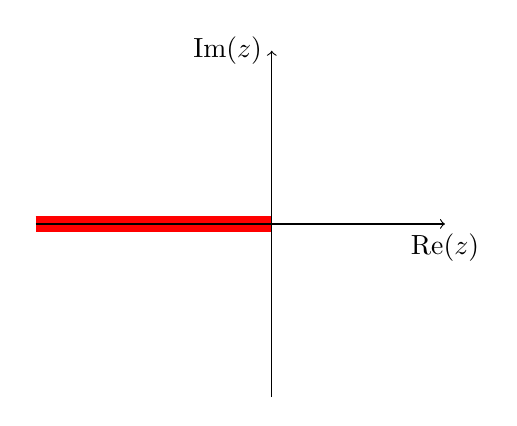
\begin{tikzpicture}[xscale=1,yscale=1]
\draw [line width=0.2cm,red] (-3.0,0) -- (0,0);
\draw [thin,->] (-3.0,0) -- (2.2,0) node [below] {Re($z$)};
\draw [thin,->] (0,-2.2) -- (0,2.2) node [left] {Im($z$)};
%=============================================
\end{tikzpicture}
\bicaption[Fig:A0Stable]{}{$\text{A}_0$稳定域}{Fig.$\!$}{Domain of $\text{A}_0$-stability}
\end{figure}

从上述稳定性定义可以得出
\begin{itemize}
\item[\ddag] A$(\pi/2)$稳定性$\iff$A稳定性。
\item[\ddag] L稳定性$\Longrightarrow$A$(\alpha)$稳定性$\Longrightarrow$A$(0)$稳定性$\Longrightarrow$$\text{A}_0$稳定性。
\end{itemize}

$\text{A}_0$稳定的算法族中包含于A稳定和A$(\alpha)$稳定的算法族中,通过详细研究$\text{A}_0$算法的性质,将能够确定合适的求解刚性微分方程的数值算法必须具备的一些条件,这也是研究$\text{A}_0$稳定性的理论意义。另一方面,许多实际的刚性问题可能只具有实的特征值,于是$\text{A}_0$稳定的算法对于求解一些特殊的刚性方程是有效的。

上述的定义只考虑了稳定性,没有考虑精度问题,Gear定义了另外可代替A稳定性的刚性稳定性\cite{Gear1971c}。即考虑了稳定性,又考虑了数值逼近的精度。其定义如下
\begin{definition}[刚性稳定的]
一个数值算法是刚性稳定的\cite{Gear1971c},如果在复平面区域$R_1\triangleq\{z:\text{Re}(z)\le D\}$它是绝对稳定的;而在区域$R_2\triangleq\{z:D<\text{Re}(z)<\alpha,|\text{Im}(z)|<\theta\}$它是精确的。
\end{definition}%\vspace{-15pt}
其在复平面内的示意图如图\ref{Fig:StifflyStable}所示,
\begin{figure}[htpb]
\centering
\begin{tikzpicture}[xscale=1,yscale=1]
\draw [pattern color=red,pattern=north east lines,dashed] (-2,-1) rectangle (2,1);
\draw [pattern color=blue,pattern=north west lines] (-4,-3) rectangle (-2,3);
\draw [white] (-4,-3) rectangle (-2,3);
\draw [thin,blue] (-2,-3) -- (-2,3);
\draw [thin,->] (-4.5,0) -- (3,0) node [below] {Re($z$)};
\draw [thin,->] (0,-3) -- (0,3) node [left] {Im($z$)};
\node [below left] at (-2,0) {$D$};
\node [above right] at (2,0) {$\alpha$};
\node [above right] at (0,1) {$\theta$};
\node [below right] at (0,-1) {$-\theta$};
\node [below] at (-1,0.8) {$R_2$};
\node [below] at (-3,2) {$R_1$};
%=============================================
\end{tikzpicture}
\bicaption[Fig:StifflyStable]{}{刚性稳定域}{Fig.$\!$}{Stiffly stability}
\end{figure}

刚性稳定的算法可以推导出该算法也是A$(\alpha)$稳定的,其中$\alpha=\tan^{-1}(\theta/D)$\cite{Fatunla1988a}。关于刚性稳定性定义的解释可以参见文献\inlinecite{Fatunla1988a,YuanZhaoDing1987a}。

Gupta在1976年提出了A$(\alpha,D)$稳定性,即包含了A稳定性的特点又结合了刚性稳定的性质。其定义如下
\begin{definition}[A$(\alpha,D)$稳定性]
一个数值算法是A$(\alpha,D)$稳定的\cite{Gupta1976a}$\alpha\in(0,\frac{\pi}{2})$,如果对于微分方程(\ref{eq:ch2StandardDiffSystem})的数值解$y_n$满足,当积分步长$h$给定,$n\to\infty$时,对于所有的$|\arg(-\lambda h)|<\alpha,D\le\text{Re}(h\lambda)<0,|\lambda|\neq0$以及所有的$\text{Re}(h\lambda)\le D$,都有$y_n\to0$。
\end{definition}
其在复平面内的示意图如图\ref{Fig:AalphaDStable}所示,
\begin{figure}[htpb]
\centering
\begin{tikzpicture}[xscale=1,yscale=1]
\path [pattern color=red,pattern=north east lines] (0,0) -- (-1.8,2) -- (-1.8,-2) -- (0,0);
\path [pattern color=blue,pattern=north west lines] (-1.8,-3) -- (-1.8,3) -- (-3.5,3) to [out=220,in=145] (-4,0) to [out=315,in=145] (-3.5,-3) -- (-1.8,-3);
\draw [red] (0,0) -- (-1.8,2) -- (-1.8,-2) -- (0,0);
\draw [blue] (-1.8,-3) -- (-1.8,3) -- (-3.5,3) to [out=220,in=145] (-4,0) to [out=315,in=145] (-3.5,-3) -- (-1.8,-3);
\draw [thin,->] (-4.5,0) -- (3,0) node [below] {Re($z$)};
\draw [thin,->] (0,-3) -- (0,3) node [left] {Im($z$)};
\node [below left] at (-1.8,0) {$D$};
\draw [blue,<-] (-0.2,0.23) to [out=225,in=90] (-0.3,0);
\node [left] at (-0.3,0.25) {$\alpha$};
\draw [blue,<-] (-0.2,-0.23) to [out=145,in=270] (-0.3,0);
\node [left] at (-0.3,-0.25) {$\alpha$};
%=============================================
\end{tikzpicture}
\bicaption[Fig:AalphaDStable]{}{A$(\alpha,D)$稳定域}{Fig.$\!$}{Domain of A$(\alpha,D)$ stability}
\end{figure}

其实,上述的各种放松A稳定性的稳定性定义,都可以理解为在复平面的某个区域$D$内,使其数值算法格式稳定。故可以归纳定义为$\text{A}_D$稳定性\cite{Odeh1971a},即
\begin{definition}[$\text{A}_D$稳定性]
给定在复平面内的一个区域$D$,一个数值算法是$\text{A}_D$稳定的\cite{Odeh1971a},若对于区域$D$内任意的$z\in D$都有其稳定函数的零根$w_i(z),i=1,2,\cdots,r$满足其模值小于1。
\end{definition}
可以看出,当区域D选择不同时,可以退化为前述提及的一些稳定性概念,如A$(\alpha)$稳定性、A$(\alpha,D)$稳定性等。当然我们也可以定义另外一个稳定性概念,即
\begin{definition}[$\text{A}_\infty$稳定性]
一个数值算法是$\text{A}_\infty$稳定的\cite{Odeh1971a,Fatunla1988a},如果其绝对稳定域包含无穷点($\infty$)的一个领域。
\end{definition}

另外一个强于A稳定性且适用于单步格式的稳定性概念就是S稳定性\cite{Prothero1974a}。
\begin{definition}[S稳定性]
一个单步数值算法是S稳定的\cite{Prothero1974a,Fatunla1988a},如果当其求解下列的非自治微分方程
\begin{equation}
y'(x)=\lambda(y-g(x))+g'(x)
\end{equation}
时(其中$g(x)$是任意的有界函数),对于$\forall h,h>h_0>0$和$\forall\lambda, \text{Re}(\lambda)<-\lambda_0$,其数值解$y_n$满足
\begin{equation}
||\frac{y_{n+1}-g(x_{n+1})}{y_n-g(x_n)}||<1
\end{equation}
\end{definition}
若将上述条件改为仅在$|\arg(-h\lambda)|<\alpha$下成立,则该单步方法称为是$S(\alpha)$\textbf{稳定的}\cite{Prothero1974a}。
\begin{definition}[强S稳定性]
一个S稳定的单步数值算法是强S稳定的\cite{Prothero1974a},如果当其求解下列的非自治微分方程
\begin{equation}
y'(x)=\lambda(y-g(x))+g'(x)
\end{equation}
时(其中$g(x)$是任意的有界函数),对于$\forall h>0$,当$\text{Re}(-\lambda)\to\infty$时其数值解$y_n$满足
\begin{equation}
\frac{y_{n+1}-g(x_{n+1})}{y_n-g(x_n)}\to0
\end{equation}
\end{definition}
很容易看出,当$g'(x)\equiv0$时,上述关于S稳定性的各种定义都将分别退化为单步算法的A稳定性、A$(\alpha)$稳定性和L稳定性。于是就有下列关系式,
\begin{itemize}
\item[\ddag] S稳定性$\Longrightarrow$A稳定性。
\item[\ddag] S$(\alpha)$稳定性$\Longrightarrow$A$(\alpha)$稳定性。
\item[\ddag] 强S稳定性$\Longrightarrow$强A稳定性(L稳定性)。
\end{itemize}

Axelsson给出了守恒微分方程稳定性的数值A稳定算法\cite{Axelsson1969a}。考虑如下的线性系统
\begin{equation}
\frac{d\bm{y}}{dt}=\bm{Ay},\quad \bm{y}(0)=\bm{\eta}\label{eq:LinearSysStableTheory}
\end{equation}
特别地,针对系统(\ref{eq:LinearSysStableTheory})的稳定性有如下定义
\begin{itemize}
\item 系统(\ref{eq:LinearSysStableTheory})是渐进稳定的,若$\bm(y)(t)\to0,t\to\infty$。
\item 系统(\ref{eq:LinearSysStableTheory})是稳定的,若存在一个常数$K$使得$|\bm{y}(t)|\le K|\bm{\eta}|,t\ge0$成立。
\end{itemize}
针对设计守恒系统(\ref{eq:LinearSysStableTheory})稳定性的数值算法定义了比A稳定性更具一般性的$\text{A}^0$稳定性。
\begin{definition}[$\text{A}^0$稳定性]
一个数值算法是$\text{A}^0$稳定的\cite{Axelsson1969a},如果对于固定的积分步长$h$,其对于系统(\ref{eq:LinearSysStableTheory})在第$r$步的数值解$y_{n,r}$满足
\begin{itemize}
\item[(i)] $\bm{y}_{n,r}\to0,r\to\infty$,如果系统(\ref{eq:LinearSysStableTheory})是渐进稳定的。
\item[(i)] 存在一个常数$K_1$使得$|\bm{y}_{n,r}|\le K_1|\bm{\eta}|,r\ge0$,如果系统(\ref{eq:LinearSysStableTheory})是稳定的。
\end{itemize}
\end{definition}


在结构动力学中,常常遇到的是经过有限元离散之后的二阶微分方程,故也有学者直接分析如下的二阶微分方程
\begin{equation}
y''(x)=-\lambda^2y(x),\quad \lambda,y\in\mathbb{R}
\end{equation}
对于上述二阶微分方程的线性$k$步法
\begin{equation}
\sum_{j=0}^{k}\alpha_jy_{n+j}=h^2\sum_{j=0}^{k}\beta_jf(y_{n+j}),\quad k\ge2\label{eq:ch2SecondDiffLMS}
\end{equation}
进行离散可以得到\begin{equation}
\sum_{j=0}^{k}(\alpha_j+z^2\beta_j)y_{n+j}=0,\qquad z\triangleq h\lambda
\end{equation}
同时,可以定义其稳定函数为\begin{equation}
p(w,z)=\sum_{j=0}^{k}(\alpha_j+z^2\beta_j)w^j
\end{equation}
显然,对于给定的$z$值,上述稳定函数有$k$个零根$w_j(z),j=1,2,\cdots,k$。其中,称$w_{1,2}(z)$为其主根,其他根为虚假根。
\begin{definition}[周期区间]
一个数值算法(\ref{eq:ch2SecondDiffLMS})是有周期区间$(0,Z_0^2)$的\cite{Lambert1976a},如果对于所有的$z^2\in(0,Z_0^2)$都有稳定函数的零根$w_i(z)$满足其两个主根为复共轭的,而其他虚假根的模值小于等于1。
\end{definition}
\begin{definition}[P稳定性]
一个数值算法(\ref{eq:ch2SecondDiffLMS})是P稳定的\cite{Lambert1976a},如果其周期区间是$(0,\infty)$。
\end{definition}
可以看出P稳定性实质上就是对于任意积分步长$h$,其数值解都可以保持有界振动,而不是衰减和发散。因此,尽管P稳定性的定义是由数值格式(\ref{eq:ch2SecondDiffLMS})出发的,但是根据P稳定性所含意义不难将其进行一般化的推广。

\begin{definition}[无条件稳定性]
一个数值算法(\ref{eq:ch2SecondDiffLMS})是无条件稳定的\cite{Dahlquist1978a},如果其稳定函数$p(w,z)$满足根条件。
\end{definition}
非常有意思的是,针对P稳定和无条件稳定的线性多步法,Lambert\cite{Lambert1976a}和Dahlquist\cite{Dahlquist1978a}分别独立的给出了如下的定理
\begin{theorem}
数值算法(\ref{eq:ch2SecondDiffLMS})是P稳定的/无条件稳定的,如果满足
\begin{itemize}
\item[(i)] 算法格式是隐式的,即$\beta_k\neq0$。
\item[(ii)] 算法格式能实现的最高阶数是2阶,且最高阶数的P稳定/无条件稳定的线性多步法是
\begin{equation}
y_{n+2}-2y_{n+1}+y_n=\frac{1}{4}h^2(f(y_{n+2})+2f(y_{n+2})+f(y_n))
\end{equation}
亦即对应的隐式Trapezoidal规则。
\end{itemize}
\end{theorem}

在结构动力学数值算法设计中,使用较多的还有C稳定性\cite{Wood1990e},其定义为
\begin{definition}[C稳定性]
一个数值算法是C稳定的\cite{Wood1990e},如果它是A稳定的,且对于所有的$z$值其稳定函数都存在一对模值最大的复共轭主根。
\end{definition}\vspace{2pt}

根据定义可以发现,P稳定性对应于这里C稳定性中的最大模值为1的情况。

对于上述定义的广义线性法(\ref{eq:ch2GLM})的稳定矩阵$\bm{M}(z)$,对于Runge-Kutta算法,将退化为Runge-Kutta方法的稳定函数$R(z)$,即
\begin{equation}
R(z)=1+z\bm{b}^T(\bm{I}-z\bm{A})^{-1}\bm{e}\label{eq:ch2RKpwz}
\end{equation}
该稳定函数在分析Runge-Kutta的阶数和性质时,经常会用到。

\begin{definition}[I稳定性]
Runge-Kutta方法(\ref{eq:ch2RK})是I稳定的\cite{ErnstHairer1996a},如果对于任意的$y\in\mathbb{R}$,其稳定函数$R(z)$满足\begin{equation}
|R(iy)|\le1
\end{equation}
\end{definition}
其实,Runge-Kutta法的I稳定性仅仅保证了算法在虚轴上的稳定性。

而对于线性多步法(\ref{eq:ch2lms}),其稳定矩阵$\bm{M}(z)$有如下形式
\begin{equation}
\begin{bmatrix}
\begin{BMAT}[4pt]{cccc:cccc}{cccc:cccc}
\frac{\alpha_1}{1-z\beta_0} & \cdots & \frac{\alpha_{k-1}}{1-z\beta_0} & \frac{\alpha_k}{1-z\beta_0} & \frac{\beta_1}{1-z\beta_0} & \cdots & \frac{\beta_{k-1}}{1-z\beta_0} & \frac{\beta_k}{1-z\beta_0}\\
1 & \cdots & 0 & 0 & 0 & \cdots & 0 & 0\\
\vdots & \ddots & \vdots & \vdots & \vdots & \ddots & \vdots & \vdots \\
0 & \cdots & 1 & 0 & 0 & \cdots & 0 & 0\\
\frac{\alpha_1}{1-z\beta_0} & \cdots & \frac{\alpha_{k-1}}{1-z\beta_0} & \frac{\alpha_k}{1-z\beta_0} & \frac{\beta_1}{1-z\beta_0} & \cdots & \frac{\beta_{k-1}}{1-z\beta_0} & \frac{\beta_k}{1-z\beta_0}\\
0 & \cdots & 0 & 0 & 1 & \cdots & 0 & 0\\
\vdots & \ddots & \vdots & \vdots & \vdots & \ddots & \vdots & \vdots \\
0 & \cdots & 0 & 0 & 0 & \cdots & 1 & 0\\
\end{BMAT}
\end{bmatrix}
\end{equation}

令$\rho(w)$和$\sigma(w)$分别表示线性多步法(\ref{eq:ch2lms})的第一和第二特征多项式,即
\begin{equation}
\rho(w)=w^k-\sum_{j=1}^{k}\alpha_jw^{k-j},\quad \sigma(w)=\sum_{j=0}^{k}\beta_jw^{k-j}
\end{equation}
这里的$\rho(w)$与前述分析线性多步法的零稳定时的$\rho(w)$是一致的。而且针对线性多步法,进一步有如下定理
\begin{theorem}
线性多步法(\ref{eq:ch2lms})在广义线性法(\ref{eq:ch2GLM})形式($r=2k$)下的稳定函数$p(w,z)=\det(w\bm{I}-\bm{M}(z))$可以简化为
\begin{equation}
p(w,z)=\frac{1}{1-z\beta_0}w^k(\rho(w)-z\sigma(w))\label{eq:ch2LMSPwz}
\end{equation}
\end{theorem}

\begin{proof}
参见文献\inlinecite{Jackiewicz2009a}的92页。
\end{proof}

当使用线性多步法(\ref{eq:ch2lms})在广义线性法(\ref{eq:ch2GLM})($r=k$)的表示形式下,尽管稳定矩阵$\bm{M}(z)$不同,但对应的稳定函数$p(w,z)$却是与(\ref{eq:ch2LMSPwz})一致的(相差$w^k$的因子),具体推导可以见文\inlinecite{Jackiewicz2009a}。

定义多项式\begin{equation}
\pi(w,z)\triangleq\rho(w)-z\sigma(w)\label{eq:ch2lmsCharaPoly}
\end{equation}
称为线性多步法(\ref{eq:ch2lms})的特征多项式,其定义与经典线性多步法理论框架\cite{LiShouFo2010a,Butcher2016a,Gear1971c,ErnstHairer1993a,ErnstHairer1996a,Butcher1987a,Fatunla1988a,YuanZhaoDing1987a}下推导的结果是一致。

对于One-leg方法(\ref{eq:ch2Oneleg}),其稳定矩阵$\bm{M}(z)$可表示为
\begin{equation}
\bm{M}(z)=\begin{bmatrix}
m_{11}(z) & \cdots & m_{1,k-1}(z) & m_{1,k}(z)\\
1 & \cdots & 0 & 0\\
\vdots & \ddots & \vdots & \vdots\\
0 & \cdots & 1 & 0\\
\end{bmatrix}
\end{equation}
其中,\begin{equation}
m_{i,j}(z)=\alpha_j+\frac{z}{1-z\beta_0}(\beta_0\alpha_j+\beta_j),\quad j=1,2,\cdots,k
\end{equation}
稳定函数$p(w,z)$为\begin{equation}
p(w,z)=\frac{1}{1-z\beta_0}(\rho(w)-z\sigma(w))
\end{equation}
关于其他数值方法在广义线性法(\ref{eq:ch2GLM})的表出形式下的稳定矩阵和稳定函数的推导可以参见文献\inlinecite{Jackiewicz2009a}。

%===============================================================================
\subsection{Runge-Kutta法的代数稳定性}
这一小节,主要给出关于Runge-Kutta方法(\ref{eq:ch2RK})的一些代数稳定性概念。

首先考虑如下的一个线性的非自治微分方程\begin{equation}
y'(t)=\xi(t)y(t),\quad y(0)=y_0\label{eq:ch2NonAutoDiffSys}
\end{equation}
其中,$\text{Re}(\xi(t))\le0$,且$\xi(t)$是任意变化的复值函数。当使用Runge-Kutta方法求解上式,则有
\begin{equation}
y_{n+1}=(1+\bm{b}^T\xi(\bm{I}-\bm{A\xi})^{-1}\bm{e})y_n
\end{equation}
其中,对角矩阵$\bm{\xi}\in\mathbb{C}^{s\times s}$的显式为
\begin{equation}
\bm{\xi}=\text{diag}(\xi_1,\cdots,\xi_s)=\text{diag}(h\xi(t_n+c_ih),\cdots,h\xi(t_n+c_sh))\label{eq:ch2Matrixi}
\end{equation}
令
\begin{equation}
K(\xi)=1+\bm{b}^T\xi(\bm{I}-\bm{A\xi})^{-1}\bm{e}
\end{equation}
于是,根据正对上式线性非自治微分方程的求解,可定义AN稳定性。特别地,当$\bm{\xi}=z\bm{I}$时,函数$K(\xi)$将退化为Runge-Kutta方法的稳定函数(\ref{eq:ch2RKpwz}),因此可以得到

AN稳定性$\Longrightarrow$A稳定性。反之不成立。
\begin{definition}[AN稳定性]
Runge-Kutta方法(\ref{eq:ch2RK})是AN稳定的,如果每当$c_i=c_j$时,对所有的$\bm{\xi}=\text{diag}(\xi_1,\cdots,\xi_s)$有$\xi_i=\xi_j$且有$\text{Re}(\xi_i)\le0,i=1,2,\cdots,s $都有函数$K(\xi)$满足
\begin{equation}
|K(\xi)|\le1
\end{equation}
\end{definition}

考虑如下一个Runge-Kutta法,其Butcher表格表示为\begin{equation}
\begin{BMAT}[5pt]{c|c}{c|c}
c & A\\  & b^T
\end{BMAT}=\begin{BMAT}[5pt]{c|cc}{cc|c}
\frac{1}{4} & \frac{1}{8} & \frac{1}{8}\\
\frac{3}{4} & \frac{3}{8} & \frac{3}{8}\\
 & \frac{1}{2} & \frac{1}{2}\\
\end{BMAT}
\end{equation}
经过简单的计算,可以发现其稳定函数$R(z)$和$K(\xi)$分别为
\begin{align}
R(z)&=\frac{2+z}{2-z}\\
K(\xi)&=\frac{8+3\xi_1+\xi_2}{8-\xi_1-3\xi_2}
\end{align}
可以证明,该Runge-Kutta法是A稳定的而非AN稳定的,因为当$\text{Re}(\xi_1),\text{Re}(\xi_2)\le0$时,其函数$K(\xi)$并非有界。

接着考虑更加一般的微分方程\begin{equation}
y'(t)=f(y(t)),\ f:\mathbb{R}^m\to\mathbb{R}^m\label{eq:ch2testfunBstable}
\end{equation}
且微分方程满足对于任意的$y,z\in\mathbb{R}^m$都有
\begin{equation}
<f(y)-f(z),y-z>\le0\label{eq:ch2OndsideLipsc}
\end{equation}
其中,“$<\cdot>$”表示在$\mathbb{R}^m$上的内积。同时BN稳定性与如下的非自治微分方程有关\begin{equation}
y'(t)=f(t,y(t)),\ f:\mathbb{R}\times \mathbb{R}^m\to\mathbb{R}^m\label{eq:ch2testfunBNstable}
\end{equation}
令$\{y_n\}_{n=0}^\infty$表示使用Runge-Kutta法(\ref{eq:ch2RK})求解系统(\ref{eq:ch2testfunBstable})在初值为$y_0$的数值解;而使用$\{\tilde{y}_n\}_{n=0}^\infty$表示使用Runge-Kutta法(\ref{eq:ch2RK})求解系统(\ref{eq:ch2testfunBstable})在初值为$\tilde{y}_0$的数值解。实质上,也可以理解$\{\tilde{y}_{n=0}^\infty\}$为$\{y_n\}_{n=0}^\infty$在初值扰动下的数值解。
\begin{definition}[B稳定性]
Runge-Kutta方法(\ref{eq:ch2RK})是B稳定的\cite{Butcher1975a,Fatunla1988a},如果针对满足条件(\ref{eq:ch2OndsideLipsc})的微分方程(\ref{eq:ch2testfunBstable})的数值解$y_n,\tilde{y}_n$,有
\begin{equation}
||y_{n+1}-\tilde{y}_{n+1}||\le||y_n-\tilde{y}_n||
\end{equation}成立。
\end{definition}

文\inlinecite{Butcher1975a}中主要分析了隐式的Runge-Kutta方法满足B稳定性的要求和条件。同时,也知道了B稳定性是A稳定性对于非线性系统分析的扩展。
\begin{definition}[BN稳定性]
Runge-Kutta方法(\ref{eq:ch2RK})是BN稳定的\cite{Butcher1975a,Fatunla1988a},如果针对满足条件(\ref{eq:ch2OndsideLipsc})的非自治微分方程(\ref{eq:ch2testfunBNstable})的数值解$y_n,\tilde{y}_n$,有
\begin{equation}
||y_{n+1}-\tilde{y}_{n+1}||\le||y_n-\tilde{y}_n||
\end{equation}成立。
\end{definition}

对于线性非自治微分方程,BN稳定性$\Longrightarrow$A、AN和B稳定性。

定义如下形式的$\bm{M}$矩阵
\begin{equation}
\bm{M}=\bm{BA}+\bm{A}^T\bm{B}-\bm{b}^T\bm{b}
\end{equation}
其中,矩阵$\bm{A}$和向量$\bm{b}$分别为Runge-Kutta法的系数,而矩阵$\bm{B}$被定义如下\begin{equation}
\bm{B}=\text{diag}(b_1,b_2,\cdots,b_s)
\end{equation}\vspace{-1.3cm}
\begin{definition}[代数稳定性]
Runge-Kutta方法(\ref{eq:ch2RK})是代数稳定的\cite{Jackiewicz2009a,Fatunla1988a},如果矩阵$\bm{B}$和矩阵$\bm{M}$都是非负定的。
\end{definition}

下列的定理给出了各个稳定性概念之间的关系。
\begin{theorem}[\inlinecite{Jackiewicz2009a}]
Runge-Kutta法(\ref{eq:ch2RK})是代数稳定的,则它也是BN稳定的。
\end{theorem}
这个定理说明了定义代数稳定性概念的意义。进一步的有
\begin{theorem}[\inlinecite{Fatunla1988a}]
一个代数稳定的Runge-Kutta法(\ref{eq:ch2RK})也是AN稳定的。如果$c_i,i=1,2,\cdots,s$互不相同,则一个AN稳定的Runge-Kutta法也是代数稳定的。
\end{theorem}

上述定理的一个推论就是
\begin{corollary}
当Runge-Kutta法中的$c_i,i=1,2,\cdots,s$互不相同时,则有

AN稳定性$\iff$BN稳定性。
\end{corollary}
而这个推论的实际含义就是它将非线性问题的稳定性直接与线性问题的稳定性建立起了联系。

通过前述提及的各种稳定性定义,可以发现不同的稳定性概念定义是基于不同的测试微分方程而定的。故这里表\ref{Tab:TestFunctionOfDiffStable}总结了各种稳定性定义所对应的测试微分方程。\vspace{-10pt}
\begin{table}[htbp]
\bicaption[Tab:TestFunctionOfDiffStable]{}{各种稳定性定义所对应的测试微分方程}{Table$\!$}{Test differential equations for stability criteria}
\vspace{0.5em}\centering\wuhao
\begin{tabular}{cc}
\toprule[1.5pt]
测试微分方程 & 稳定性准则\\
\midrule[1pt]
$y'(t)=\lambda y(t)$ & A稳定性、L稳定性\\
$y'(t)=\lambda(t) y(t)$ & AN稳定性、LN稳定性\\
$y'(t)=f(y(t))$ & B稳定性\\
$y'(t)=f(t,y(t))$ & BN稳定性、B稳定性\\
$y'(t)=\lambda(y(t)-g(t))+g'(t)$ & S稳定性\\
$\bm{y}'(t)=\bm{A}(t)\bm{y}(t)$ & D稳定性\\
$y''(t)=\omega^2y(t)$ & P稳定性、C稳定性\\
\bottomrule[1.5pt]
\end{tabular}
\end{table}
%==================================================================================
\subsection{广义线性法的代数稳定性}
对微分方程(\ref{eq:ch2NonAutoDiffSys})使用广义线性法(\ref{eq:ch2GLM})求解可得
\begin{equation}
y^{[n+1]}=\bm{S}(\bm{\xi})y^{[n]}
\end{equation}
其中,$\bm{\xi}$由前述定义(\ref{eq:ch2Matrixi})计算,且$\bm{S}(\bm{\xi})$的显式表达为\begin{equation}
\bm{S}(\bm{\xi})=\bm{V}+\bm{B\xi}(\bm{I}-\bm{A\xi})^{-1}\bm{U}
\end{equation}

令矩阵$\bm{G}=[g_{ij}]_{i,j=1}^r$是实对称正定矩阵,对于向量$y\in\mathbb{R}^{mr}$\begin{equation}
y=\begin{bmatrix}
y_1\\ y_2\\ \vdots \\ y_r
\end{bmatrix},\quad y_i\in\mathbb{R}^m,\quad i=1,2,\cdots,r
\end{equation}
定义如下的G范数
\begin{equation}
||y||_G^2=\sum_{i=1}^{r}\sum_{j=1}^{r}g_{ij}y_i^Ty_j
\end{equation}

于是,可以根据G范数可以定义广义线性法的AN稳定性。
\begin{definition}[AN稳定性]
广义线性法(\ref{eq:ch2GLM})是AN稳定的\cite{Jackiewicz2009a},如果每当$c_i=c_j$时,对所有的$\bm{\xi}=\text{diag}(\xi_1,\cdots,\xi_s)$有$\xi_i=\xi_j$且在$\text{Re}(\xi_i)\le0,i=1,2,\cdots,s $成立时,存在一个实对称正定矩阵$\bm{G}$使得
\begin{equation}
||\bm{S}(\bm{\xi})y||_G\le||y||_G
\end{equation}成立。
\end{definition}
对于广义线性法的AN稳定性的其他等价定义可以参加文献\inlinecite{Butcher1987a}。当$\bm{\xi}=z\bm{I}$成立时,矩阵$\bm{S}(\bm{\xi})$将退化为广义线性法的稳定矩阵$\bm{M}(z)$,因此一个广义线性法是AN稳定的,那么它也是A稳定的。

同样地,令$\{y^{[n]}\}_{n=0}^\infty$和$\{\tilde{y}^{[n]}\}_{n=0}^\infty$表示广义线性法(\ref{eq:ch2GLM})求解带有不同初值问题的微分方程(\ref{eq:ch2testfunBstable})的数值解。则可以定义广义线性法的G稳定性
\begin{definition}[G稳定性]
广义线性法(\ref{eq:ch2GLM})是G稳定的\cite{Jackiewicz2009a},如果对于所有满足条件(\ref{eq:ch2OndsideLipsc})的微分方程(\ref{eq:ch2testfunBNstable})在两个不同初值条件下的数值解$\{y^{[n]}\}_{n=0}^\infty$和$\{\tilde{y}^{[n]}\}_{n=0}^\infty$有存在一个实对称正定矩阵$\bm{G}$使得
\begin{equation}
||y^{[n+1]}-\tilde{y}^{[n+1]}||_G\le||y^{[n]}-\tilde{y}^{[n]}||_G
\end{equation}成立。
\end{definition}

类似于Runge-Kutta法,对于给定的矩阵$\bm{G}\in\mathbb{R}^{r\times r}$和矩阵$\bm{D}\in\mathbb{R}^{s\times s}$,定义其矩阵$\bm{M}$为
\begin{equation}
\bm{M}\triangleq\begin{bmatrix}
\begin{BMAT}[5pt]{c|c}{c|c}
\bm{DA}+\bm{A}^T\bm{D}-\bm{B}^T\bm{GB} & \bm{DU}-\bm{B}^T\bm{GV}\\
\bm{U}^T\bm{D}-\bm{V}^T\bm{GB} & \bm{G}-\bm{V}^t\bm{GV}\\
\end{BMAT}
\end{bmatrix}\label{eq:GLMG}
\end{equation}

有了矩阵$\bm{M}$的定义,就可以很方便的定义广义线性法的代数稳定性。
\begin{definition}[代数稳定性]
广义线性法(\ref{eq:ch2GLM})是代数稳定的\cite{Jackiewicz2009a},如果存在一个实对称正定矩阵$\bm{G}$和实对角正定矩阵$\bm{D}$使得等式(\ref{eq:GLMG})中的矩阵$\bm{M}$是非负定的。
\end{definition}

由此可见,对于证明一个广义线性法是代数稳定的的,需要找到矩阵$\bm{G,D}$,同时文\inlinecite{Burrage1980b}已经证明对于预相容且代数稳定的广义线性法(\ref{eq:ch2GLM}),其矩阵$\bm{G},\bm{D}$并非相互独立而是由下列的等式相关联
\begin{equation}
\bm{De}=\bm{B}^T\bm{Gq}_0
\end{equation}
其中,$\bm{q}_0$是预相容向量。而且,向量$\bm{Gq}_0$是系数矩阵$\bm{V}$的特征值1所对应的左特征向量,即
\begin{equation}
(\bm{I}-\bm{V}^T)\bm{Gq}_0=\bm{0}
\end{equation}
进一步,广义线性法的各个稳定性之间的关系如下

代数稳定性$\Longrightarrow$G稳定性$\Longrightarrow$AN稳定性$\Longrightarrow$A稳定性。

上述的关系仅仅是单向的,如果加上一些条件,可以得到如下的结果
\begin{theorem}[\inlinecite{ErnstHairer1996a}]
对于预相容的广义线性法(\ref{eq:ch2GLM}),且$c_i,i=1,2,\cdots,s$互不相同,则有:代数稳定性$\iff$G稳定性$\iff$AN稳定性。
\end{theorem}
%========================================================================

\section{收敛性}
正如线性多步法一样,在进行数值方法的应用之前,往往需要启动方法进行初始计算。而广义线性法也需要一个特殊的启动机制来完成$r$维向量$\bm{y}^{[n]}$的装配工作。但这里我们不准备详细阐述其原理,详见文献\inlinecite{Califano2017a,Butcher2016a}。本文假定存在一个带有积分步长$h$的启动机制$\bm{S}_h$
\begin{equation}
\bm{S}_h:\mathbb{R}^{m}\to\mathbb{R}^{mr}
\end{equation}
使得初始向量$y^{[0]}=y^{[0]}(h)\in\mathbb{R}^{mr}$转换为
\begin{equation}
\lim_{h\to0}\bm{S}_h(y_0)=\lim_{h\to0}y^{[0]}=(\bm{q}_0\otimes\bm{I})y(t_0)\label{eq:Sh}
\end{equation}
其中,$\bm{q}_0$是某个预相容向量。而$y_0\in\mathbb{R}^m$是初始值,$y(t)$是微分方程(\ref{eq:ch2FirstAuto})的解。
\begin{definition}[收敛性定义]
广义线性法($\bm{c},\bm{A},\bm{U},\bm{B},\bm{V}$)是收敛的,如果对于任意满足Lipschitz条件的微分方程(\ref{eq:ch2FirstAuto}),存在一个非零向量$\bm{q}_0$和一个满足条件(\ref{eq:Sh})启动机制$\bm{S}_h$,使得对于任意的$\overline{t}\in[t_0,T]$和$h=(\overline{t}-t_0)/n$下,由广义线性法(\ref{eq:ch2GLM})在$y^{[0]}=\bm{S}_h(y_0)$下计算$n$步得到的向量$y^{[n]}$收敛到$\bm{q}_0y(\overline{t})$,其中,$y(t)$是微分方程(\ref{eq:ch2FirstAuto})的一个解。
\end{definition}
需要说明的是,上述针对广义线性法的定义也适用于线性多步法。因为通过前述线性多步法(\ref{eq:ch2lms})在广义线性法(\ref{eq:ch2GLM})的表示形式,上述稳定性定义可以很容易的与经典线性多步法的理论下的稳定性定义做对比。

在线性多步法的经典理论中,我们可以知道,其收敛性可以由相容性和稳定性保证,即
\begin{center}
\textbf{相容性+稳定性=收敛性 }
\end{center}

其实,在广义线性法中也有类似的收敛性条件,即,\textbf{零稳定性+相容性=收敛性 }。
\begin{theorem}
若广义线性法($\bm{c},\bm{A},\bm{U},\bm{B},\bm{V}$)是收敛的,则它是零稳定的和相容的。
\end{theorem}
\begin{proof}
首先,使用反证法证明收敛性暗示零稳定性。假定序列$||\bm{V}^n||,n=1,2,\cdots$是无界的。因为下式关系存在
\begin{equation}
||\bm{V}^n||=\max_{||w||=1}||\bm{V}^nw||,\ n=1,2,\cdots
\end{equation}
则存在一个向量序列$w_n,(||w_n||=1)$使得序列$||\bm{V}^nw_n||,n=1,2,\cdots$也是无界的。考虑如下的微分方程
\begin{equation}
y'(t)=0,\quad y(0)=0
\end{equation}
且$t\in[0,1]$。当积分步长$h=1/n$时,其初始向量$y^{[0]}$可由如下给出
\begin{equation}
y^{[0]}=\bm{S}_h(0)=\frac{w_n}{\max\limits_{1\le i\le n}||\bm{V}^iw_i||}
\end{equation}
由于序列$\bm{V}^nw_n$是无界的,因此有$\lim_{h\to0}\bm{S}_h(0)=0$。而在$n$次积分步之后有
\begin{equation}
y^{[n]}=\bm{V}^n\bm{S}_h(0)=\frac{\bm{V}^nw_n}{\max\limits_{1\le i\le n}||\bm{V}^iw_i||}
\end{equation}
且其范数为
\begin{equation}
||y^{[n]}||=||\bm{V}^n\bm{S}_h(0)||=\frac{||\bm{V}^nw_n||}{\max\limits_{1\le i\le n}||\bm{V}^iw_i||}
\end{equation}
因为$||\bm{V}^nw_n||$是无界的,因此存在一个连续递增的子序列$||\bm{V}^{n_j}w_{n_j}||$使得$\lim\limits_{j\to\infty}||\bm{V}^{n_j}w_{n_j}||=\infty$和$\max\limits_{1\le i\le n_j}||\bm{V}^iw_i||=||\bm{V}^{n_j}w_{n_j}||$。于是,就有
\begin{equation}
||y^{[n_j]}||=|\bm{V}^{n_j}\bm{S}(1/n_j)||=1\neq 0
\end{equation}
这与广义线性法的收敛性相矛盾。

下证,收敛性暗示相容性。考虑如下的初值问题
\begin{equation}
y'(t)=1,\quad y(0)=0
\end{equation}
且$t\in[0,1]$。取积分步长为$h=1/n$,而初始向量为$y^{[0]}$由
\begin{equation}
y^{[0]}=\bm{S}_h(0)=\bm{q}_0y(0)=\bm{0}
\end{equation}
给出。而第$i$步调输出向量为
\begin{equation}
y^{[i]}=h\bm{Be}+\bm{V}y^{[i-1]},\quad i=1,2,\cdots,n
\end{equation}
于是就有
\begin{equation}
y^{[n]}=h(\bm{I}+\bm{V}+\cdots+\bm{V}^{n-1})\bm{Be}
\end{equation}
因为$\bm{V}^i\bm{q}_0=\bm{q}_0,i=0,1,\cdots$,进而
\begin{equation}
h(\bm{I}+\bm{V}+\cdots+\bm{V}^{n-1})\bm{q}_0=hn\bm{q}_0=\bm{q}_0
\end{equation}
可以得出
\begin{equation}
y^{[n]}-\bm{q}_0=h(\bm{I}+\bm{V}+\cdots+\bm{V}^{n-1})(\bm{Be}-\bm{q}_0)
\end{equation}

因为系数矩阵$\bm{V}$稳定的,故存在一个非奇异矩阵$\bm{P}$使得
\begin{equation}
\bm{V}=\bm{P}^{-1}\begin{bmatrix}
\begin{BMAT}[5pt]{cc}{cc}
\bm{I} & \bm{0}\\
\bm{0} & \tilde{\bm{V}}
\end{BMAT}
\end{bmatrix}\bm{P}
\end{equation}
其中,矩阵$\bm{I}$是$\tilde{r}\times\tilde{r}$维的单位矩阵,而$\tilde{\bm{V}}$是稳定的,且其特征值不含$1$。于是又有\begin{equation}
\begin{aligned}
y^{[n]}-\bm{q}_0&=\bm{P}^{-1}\begin{bmatrix}
\begin{BMAT}[5pt]{cc}{cc}
\bm{I} & \bm{0}\\
\bm{0} & h(\bm{I}+\tilde{\bm{V}}+\cdots+\tilde{\bm{V}^{n-1}})
\end{BMAT}
\end{bmatrix}\bm{P}(\bm{Be}-\bm{q}_0)\\
&=\bm{P}^{-1}\begin{bmatrix}
\begin{BMAT}[5pt]{cc}{cc}
\bm{I} & \bm{0}\\
\bm{0} & h(\bm{I}-\tilde{\bm{V}})^{-1}(\bm{I}-\tilde{V}^n)
\end{BMAT}
\end{bmatrix}\bm{P}(\bm{Be}-\bm{q}_0)
\end{aligned}\label{eq:ch2conven}
\end{equation}
同时,考虑第$n$步输出量$y^{[n]}$的极限值,即
\begin{equation}
\lim_{n\to\infty,hn=1}y^{[n]}=\bm{q}_0y(1)=\bm{q}_0
\end{equation}
进而等式(\ref{eq:ch2conven})可转换为
\begin{equation}
\begin{bmatrix}
\begin{BMAT}[5pt]{cc}{cc}
\bm{I} & \bm{0}\\
\bm{0} & \bm{0}
\end{BMAT}
\end{bmatrix}\bm{P}(\bm{Be}-\bm{q}_0)=\begin{bmatrix}
\begin{BMAT}[5pt]{c}{cc}
 \bm{0}\\
\bm{0}
\end{BMAT}
\end{bmatrix}
\end{equation}
这表明向量$\bm{P}(\bm{Be}-\bm{q}_0)$在它的前$\tilde{r}$个分量中全为0。因为矩阵$\bm{I}-\tilde{\bm{V}}$是非奇异的,因此可以将向量$\bm{P}(\bm{Be}-\bm{q}_0)$改写为如下形式
\begin{equation}
\bm{P}(\bm{Be}-\bm{q}_0)=\begin{bmatrix}
\begin{BMAT}[5pt]{c}{cc}
 \bm{0}\\
(\bm{I}-\tilde{\bm{V}})\tilde{\bm{q}}_1
\end{BMAT}
\end{bmatrix}
\end{equation}
其中,$\tilde{\bm{q}}_1\in\mathbb{R}^{r-\tilde{r}}$。定义向量$\bm{q}_1\in\mathbb{R}^r$如下
\begin{equation}
\bm{q}_1=\bm{P}^{-1}\begin{bmatrix}
\begin{BMAT}[5pt]{c}{cc}
 \bm{0}\\
\tilde{\bm{q}}_1
\end{BMAT}
\end{bmatrix}
\end{equation}
于是就有
\begin{equation}
\begin{aligned}
\bm{P}(\bm{Be}-\bm{q}_0)&=\begin{bmatrix}
\begin{BMAT}[5pt]{cc}{cc}
\bm{I} & \bm{0}\\
\bm{0} & \bm{I}-\tilde{\bm{V}}
\end{BMAT}
\end{bmatrix}\begin{bmatrix}
\begin{BMAT}[5pt]{c}{cc}
 \bm{0}\\
\tilde{\bm{q}}_1
\end{BMAT}
\end{bmatrix}\\
&=\left(\bm{I}-\begin{bmatrix}
\begin{BMAT}[5pt]{cc}{cc}
\bm{I} & \bm{0}\\
\bm{0} & \tilde{\bm{V}}
\end{BMAT}
\end{bmatrix}\right)\bm{P}\bm{q}_1\\
&=\bm{P}\left(\bm{I}-\bm{P}^{-1}\begin{bmatrix}
\begin{BMAT}[5pt]{cc}{cc}
\bm{I} & \bm{0}\\
\bm{0} & \tilde{\bm{V}}
\end{BMAT}
\end{bmatrix}\bm{P}\right)\bm{q}_1\\
&=\bm{P}(\bm{I}-\bm{V})\bm{q}_1
\end{aligned}
\end{equation}
因此可得$\bm{Be}+\bm{Vq}_1=\bm{q}_0+\bm{q}_1$,就是相容性条件。完成了证明。
\end{proof}

在证明零稳定性和相容性可以推导出收敛性之前,需要如下的引理。
\begin{lemma}[\inlinecite{Jackiewicz2009a}]
若矩阵$\bm{A}\in\mathbb{R}^{r\times r}$是稳定的(其有界常数为$C_1\ge1$)。两个序列$u_n,w_n\in\mathbb{R}^r$满足如下关系
\begin{equation}
u_n=\bm{A}u_{n-1}+w_n,\quad ||w_n||\le C_2||u_{n-1}||+\delta,\ n=0,1,2,\cdots
\end{equation}
其中,常数$C_2\ge0,\delta\ge0$。则有
\begin{equation}
||u_n||\le C_1(1+C_1C_2)^n||u_0||+\frac{\delta}{C_2}\left((1+C_1C_2)^n-1\right),\ C_2>0,n=0,1,2,\cdots
\end{equation}
若$C_2=0$,则对上式右端取极限既可,即得$C_1(||u_0||+n\delta)$。
\end{lemma}
\begin{proof}
参见文献\inlinecite{Jackiewicz2009a}。
\end{proof}

\begin{theorem}[\inlinecite{Jackiewicz2009a,Butcher2016a}]
一个零稳定的且相容的广义线性法($\bm{c},\bm{A},\bm{U},\bm{B},\bm{V}$)是收敛的。
\end{theorem}
\begin{proof}
参见文献\inlinecite{Jackiewicz2009a,Butcher2016a}。
\end{proof}










\section{精度分析}

\subsection{数值耗散}

\subsection{数值弥散}

\section{超调行为}

\section{虚假根分析}

\section{直接积分法的放大矩阵}

\begin{definition}
直接积分算法的一致性\cite{Hoff1988c}。如果两个直接积分算法的放大矩阵$A$的对应元素分别相等\footnote{这也是矩阵相等的定义。},则称这两个积分算法是一致的。
\end{definition}

\begin{definition}
直接积分算法的相似性/谱等价\cite{Hoff1988c}。如果两个直接积分算法的放大矩阵$A$的不变量分别对应相等,则称这两个积分算法是相似的/谱等价的。
\end{definition}

需要说明的是,一般情况下,两个谱等价的算法并不一定能导出一致的数值算法特性;而两个算法的一致性可以保证。这样的例子可以参见文献\inlinecite{Hoff1988b}。

\section{本章小结}


